\documentclass[]{article}

\usepackage{caption,subcaption,graphicx,float,url,amsmath,amssymb,amsthm,tocloft,cancel,mathrsfs}
\usepackage[toc,nonumberlist]{glossaries}
\usepackage{glossaries-extra,thmtools,gensymb,braket,bm,tensor}
\usepackage[toc,page]{appendix}

\newcommand\numberthis{\addtocounter{equation}{1}\tag{\theequation}}
\newcommand{\Lagr}{\mathscr{L}}
\newtheorem{thm}{Theorem}
\newtheorem{defn}[thm]{Definition}
\newtheorem{cor}[thm]{Corollary}
\newtheorem{lemma}[thm]{Lemma}
\graphicspath{{figs/}}
\widowpenalty10000
\clubpenalty10000
\setcounter{tocdepth}{2}

%opening
\title{Theoretical Minimum\\General Relativity}
\author{}

\begin{document}

\maketitle

\begin{abstract}
	These are my notes for the \emph{General Relativity}\cite{susskind2012general} lectures from Leonard Susskind's \emph{Theoretical Minimum} series\cite{susskind2007theoretical}.
\end{abstract}

\tableofcontents
\listoffigures
\listoftables
\listoftheorems

\section{The Equivalence Principle \& Tensor Analysis}

LS begins where Einstein started. Einstein started with the simplest things and deduced far racing conclusions.

\subsection{The Equivalence Principle}

This is the principle that gravity is, in some sense, the same as acceleration.

\subsubsection{Coordinate Transformations}

If we are in an accelerated frame of reference, an elevator moving up or down say, we feel a gravitational field. Children know that.

Figure \ref{fig:gr-1-elevator} depicts an elevator. Assuming we know the laws of physics in the $z$ frame, surely we can figure then out in $z^\prime$.

\begin{figure}[H]
	\begin{center}
		\caption[Moving Elevator]{Moving Elevator: there are two coordinate systems, $z$ and $z^\prime$, and $L(t)$ allows us to pass from one to the other.}\label{fig:gr-1-elevator}
		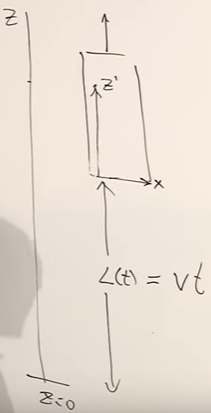
\includegraphics[width=0.4\textwidth]{gr-1-elevator}
	\end{center}
\end{figure}

In this lecture we'll ignore Special Relativity, which is tantamount to setting $c=\infty$ or assuming all velocities very small. If General Relativity is the generalization of Special Relativity, how did Einstein get away with ignoring Special Relativity? The answer is that Special Relativity is about high velocities. Gravity has to do with heavy masses. There are situation where the mass is high, but the velocity isn't. Einstein started thinking about these situations, and then combined it with Special Relativity to think about the combination of high masses and high velocities.

Let's think about inertial reference frames. If $z$ and $z^\prime$ are inertial, they are related by uniform velocity, so we have the coordinate transformation:

\begin{align*}
	L(t)=&vt\\
	z^\prime =& z-L(t)\\
	=& z-vt\\
	t^\prime =& t\\
	x^\prime =& x
\end{align*}

Now introduce Newton's 2nd law of motion. How does this change under the coordinate transformation?

\begin{align*}
	F =& m \ddot{z} \text{ in the $z$ frame}\\
	\ddot{z^\prime} =& \ddot{z} \text{ since $v$ is constant, whence:}\\
	F =& m \ddot{z^\prime} \text{ since $v$ is constant, so Newton's 2nd Law holds.}
\end{align*}

Now let's go to an accelerated frame--Figure \ref{fig:gr-1-elevator-accelerated}.

\begin{figure}[H]
	\begin{center}
		\caption{Elevator in a accelerated Frame}\label{fig:gr-1-elevator-accelerated}
		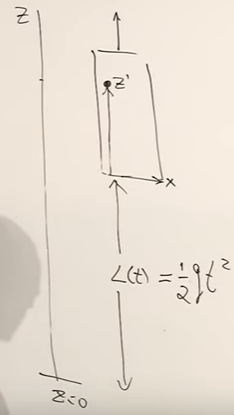
\includegraphics[width=0.4\textwidth]{gr-1-elevator-accelerated}
	\end{center}
\end{figure}

The coordinate transformation is now:
\begin{align*}
	L(t)=&vt\\
	z^\prime =& z-\frac{1}{2}g t^2\\
	=& z-vt\\
	t^\prime =& t\\
	x^\prime =& x
\end{align*}

We will continue to assume that Newton's laws hold in the $z$ frame of reference.
\begin{align*}
	\ddot{z^\prime} =& \ddot{z}-g\\
	\underbrace{F -mg}_\text{Force, including fictitious term} =& m \ddot{z^\prime} 
\end{align*}

The fictitious force looks like a uniform gravitational field. The special property of gravity is that gravitational forces are proportional to mass. That has a deep implication: the mass cancels, so the motion doesn't depend on the mass. Most people before Einstein considered this largely an accident. People know that acceleration mimicked gravity; Einstein said it was deep principle of nature. Figure \ref{fig:gr-1-coordinates-const} shows the coordinate transformation for constant velocity. Straight lines go to straight lines. Figure \ref{fig:gr-1-coordinates-accelerated} shows the results of accelerating the coordinate system: straight lines are not preserved. We have a curvy linear transformation. Einstein understood very early that there is a connection between gravity and curvy linear transformations of spacetime. Special Relativity was all about linear transformations\cite{susskind2017special}.

\begin{figure}[H]
	\begin{center}
		\caption{Coordinate Transformation for constant velocity versus accelerated}
		\begin{subfigure}[t]{0.45\textwidth}
			\caption{Coordinate Transformation for constant velocity. Green represents 	constant $z^\prime$}\label{fig:gr-1-coordinates-const}
			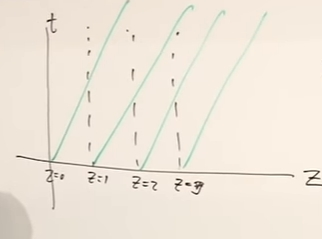
\includegraphics[width=\textwidth]{gr-1-coordinates-const}
		\end{subfigure}
		\;
		\begin{subfigure}[t]{0.4\textwidth}
			\caption{Coordinate Transformation 		accelerated}\label{fig:gr-1-coordinates-accelerated}
			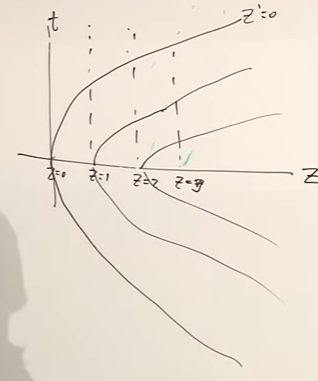
\includegraphics[width=\textwidth]{gr-1-coordinates-accelerated}
		\end{subfigure}
	\end{center}
\end{figure}



\subsubsection{Example: what is the influence of gravity on light?}
In 1907 most physicists would have thought there was no effect. Einstein argued from the equivalence principle that gravity would affect light. Consider a beam of light in our elevator--Figures \ref{fig:gr-1-light-in-elevator} and \ref{fig:gr-1-elevator-accelerated-curved-path}.

\begin{figure}[H]
	\caption{What is the influence of gravity on light? }
	\begin{subfigure}[t]{0.5\textwidth}
		\caption{Path of Light in $z$ system}\label{fig:gr-1-light-in-elevator}
		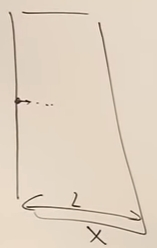
\includegraphics{gr-1-light-in-elevator}
	\end{subfigure}
	\begin{subfigure}[t]{0.5\textwidth}
		\caption{Path of Light in $z^\prime$ system}\label{fig:gr-1-elevator-accelerated-curved-path}
		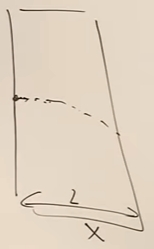
\includegraphics{gr-1-elevator-accelerated-curved-path}
	\end{subfigure}
\end{figure}

We'll write down the equation for the path of the light beam:
\begin{align*}
	x =& ct \text{ in the $z$ frame, and}\\
	z =& 0 \text{; in the moving frams}\\
	z^\prime + g\frac{t^2}{2} =&0 \text{, which is curved--Figure \ref{fig:gr-1-elevator-accelerated-curved-path}}
\end{align*}

\begin{itemize}
	\item In the primed system light is bending down;
	\item In the unprimed system the elevator is accelerating--the beam only \emph{looks} curved.
\end{itemize}

Einstein said that they are both the same thing.

What we have learned. 

\begin{enumerate}
	\item It is interesting to think about curvy linear transformations. 
	\item When you think about curvy linear transformations the form of Newton's Laws changes.
	\item One thing that happens is that apparent  gravitational fields  materialize that are apparently indistinguishable from ordinary gravitational fields.
\end{enumerate}

But are they really indistinguishable? Not really. Let's talk about gravitational fields generated by the Sun or the Earth--Figure \ref{fig:gr-1-suns-gravitational-field}. It is pretty obvious that there is no way to do a coordinate transformation like the ones we've been discussing which will remove the gravitational field. In \ref{fig:gr-1-suns-gravitational-field-local} we are in a laboratory we can transform away the field locally,  but there is no way to get rid of the fact that we are dealing with a field that is inwards globally.

\begin{figure}[H]
	\begin{center}
		\caption{Sun's Gravitational Field}
		\begin{subfigure}[t]{0.45\textwidth}
			\caption{There is no way to do a coordinate transformation like the ones we've 	been discussing which will remove the gravitational field}\label{fig:gr-1-suns-gravitational-field}
			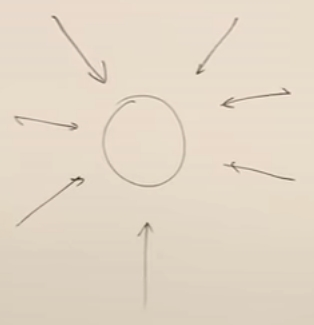
\includegraphics[width=\textwidth]{gr-1-suns-gravitational-field}
		\end{subfigure}
		\;
		\begin{subfigure}[t]{0.45\textwidth}
			\caption{If we are in a laboratory we can transform away the field locally, but 	there is no way to get rid of the fact that we are dealing with a field that is inwards globally.}\label{fig:gr-1-suns-gravitational-field-local}
			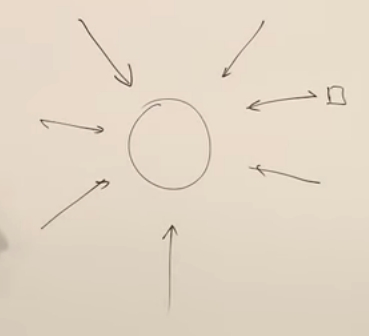
\includegraphics[width=\textwidth]{gr-1-suns-gravitational-field-local}
		\end{subfigure}
	\end{center}
\end{figure}

Figure \ref{fig:2000:mile:man} shows why we can't transform the field away. In Figure \ref{fig:gr-1-suns-gravitational-field-2000-mile-ff} 2000 Mile Man is oriented with his feet towards the Sun: he feels a tidal pull, as his feet are closer to the Sun than his head. In Figure \ref{fig:gr-1-suns-gravitational-field-2000-mile} he feels pressure at his head and feet. Being squashed is not something we can get rid of by performing a coordinate transformation. So it is not true that gravity is equivalent to a coordinate transformation. Einstein said that for small objects and small times, gravity was equivalent to a coordinate transformation.
\begin{figure}[H]
	\begin{center}
		\caption{The adventures of 2000 mile man}\label{fig:2000:mile:man}
		\begin{subfigure}[t]{0.45\textwidth}
			\caption{ 2000 Mile Man is oriented with his feet towards the Sun: he feels a 	tidal pull, as his feet are closer to the Sun than his head. }\label{fig:gr-1-suns-gravitational-field-2000-mile-ff}
			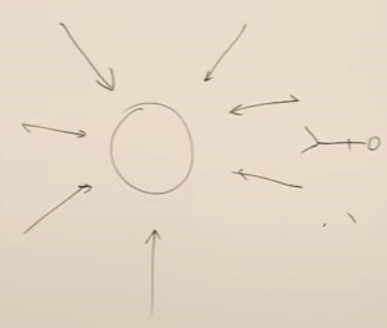
\includegraphics[width=\textwidth]{gr-1-suns-gravitational-field-2000-mile-ff}
		\end{subfigure}
		\;
		\begin{subfigure}[t]{0.45\textwidth}
			\caption{This time our hero feels pressure at his head and feet. Being squashed 	is not something we can get rid of by performing a coordinate transformation.}\label{fig:gr-1-suns-gravitational-field-2000-mile}
			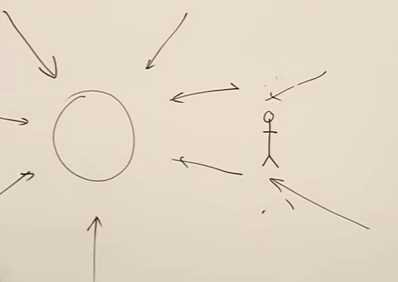
\includegraphics[width=\textwidth]{gr-1-suns-gravitational-field-2000-mile}
		\end{subfigure}
	\end{center}
\end{figure}

That raises a question: if I present you with a force field, e.g. the force field of uniform acceleration--Figure \ref{fig:gr-1-uniform-force-field}--you can make it look more complicated via a suitable transformation. If a transformation involve the $x$ axis it can make the field bend, or accelerate along $z$ while oscillating along $x$. This will give a complicated apparent gravitational field. If I tell you what the field is everywhere, how do I determine if it is just a fake gravitational field, from acceleration, or a real genuine one? If it is Newtonian gravitational field, just calculate the tidal forces on a freely falling object. If there is squeezing or stretching we have gravity,  otherwise not. If you can transform the field away it is not real gravity, otherwise it is real (can detect tidal forces via crystal).

\begin{figure}[H]
	\begin{center}
		\caption{Uniform Force Field}\label{fig:gr-1-uniform-force-field}
		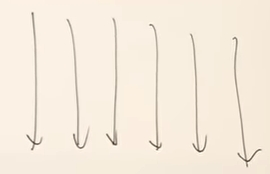
\includegraphics[width=0.5\textwidth]{gr-1-uniform-force-field}
	\end{center}
\end{figure}


Einstein asked what kind of mathematics he needed to answer the questions about real and apparent gravitational fields. The other element was special relativity: he know from the work of Minkowski that special relativity had a geometry associated with it, which had a length, proper distance.

\begin{align*}
	d\tau^2 =& dt^2 - dx^2 \text{, or, depending on who you are}\\
	ds^2 =& dx^2 -dt^2
\end{align*}

Einstein realized that the problem of deciding whether or not a gravitation field was real was similar to a problem that Riemann had explored, deciding whether or not a space was flat. Riemann had not considered metrics with a minus sign. In Euclidean space:
\begin{align*}
	ds^2 =& \sum (dx^i)^2 \numberthis \label{eq:euclidean:metric}
\end{align*}
 
Gauss had already understood that in non-Euclidean spaces the formula for distance on a surface was more complicated. Riemann took the next step. Consider a curved surface (let's not worry what this means exactly), and lay out coordinates as in Figure \ref{fig:gr-1-curved-surface-coordinates}.
 
\begin{figure}[H]
	\begin{center}
		\caption[Curved Surface with coordinates]{Curved Surface with coordinates. Don't worry about straight lines.}\label{fig:gr-1-curved-surface-coordinates}
		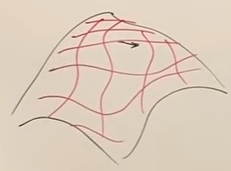
\includegraphics{gr-1-curved-surface-coordinates}
	\end{center}
\end{figure} 

The formula for the distance between two close points becomes:
\begin{align*}
	ds^2 =& \sum_{m,n} g_{mn}(x) dx^m dx^n
\end{align*}
It works also for curved coordinates in a flat space.

We are building up geometry in little regions and piecing them together. Maybe we can put them together on a flat plane, but maybe not. So, given the little pieces, how do we know whether or not it is flat? Is there a coordinate system where (\ref{eq:euclidean:metric}) holds?

We have two parallel questions. Can we find a coordinate system:
\begin{itemize}
	\item where apparent gravitational field is zero;
	\item where (\ref{eq:euclidean:metric}) is true.
\end{itemize}

We will need the mathematics of Tensor Analysis.

\subsection{Tensor Analysis}

Can we change $g_{mn}$ to $\delta_{mn}$? First question is how does $g_{mn}$ change when we change coordinates?

We have two sets of coordinates, $x$ and $y$, and write $x^m = x^m(y)$, and $y^m = y^m(x)$. How do $dx_m$ transform?

\begin{align*}
	dy^m =& \sum_p \frac{\partial y^m}{\partial x^p} dx^p\\
	V^{\prime m} =& \sum_p \frac{\partial y^m}{\partial x^p} V^p \text{, or, using Einstein's summation convention} \\
	V^{\prime m} =&  \frac{\partial y^m}{\partial x^p} V^p \numberthis \label{eq:contravariant}
\end{align*}

\begin{defn}[Contravariant]
	A Vector whose components transform in accordance with (\ref{eq:contravariant}) is said to be \emph{contravariant}.
\end{defn}

Consider a scalar function, $s$, then the gradient is a vector.

\begin{defn}[Gradient]
	The gradient of $s$ is $\frac{\partial s}{\partial x^p}$.
\end{defn}

\begin{align*}
	\frac{\partial s}{\partial y^m} =& \frac{\partial s}{\partial x^p}\frac{\partial x^p}{\partial y^m}\\
	W_m^\prime =& \frac{\partial x^p}{\partial y^m} W_p \numberthis \label{eq:covariant}
\end{align*}

\begin{defn}[Covariant]
	A Vector whose components transform in accordance with (\ref{eq:covariant}) is said to be \emph{covariant}.
\end{defn}
 
Relativity is about the transformation properties of objects.

To define more general tensors, consider products of vectors -- e.g.
\begin{align*}
	V^mU^n=&T^{mn} \text{, contravariant tensor of rank 2 }
\end{align*}

LS derived the transformation properties, and showed that $g_{mn}$ is covariant.


\section{Tensor mathematics}

A good notation will carry you a long way. When it is good it tells you what to do next. It's like tinker toys: you put the stick into a hole. The notation of GR is like that: if you follow the rules it is difficult to make mistakes. The rules are tensor analysis and tensor algebra.

\subsection{Flat space}

Our aim is to distinguish flat from not flat. LS rolls flat page into cylinder, which is locally flat (it has extrinsic curvature from the embedding in 3D, not intrinsic: a tiny bug embedded in the surface can't notice this sort of curvature, but can find intrinsic curvature). Riemannian geometry is about intrinsic properties of space.
 
Figures \ref{fig:gr-2-lattice} and \ref{fig:gr-2-lattice-not-flat} illustrate a surface can be flattened and one that cannot. A curved surface is one that cannot be flattened without distorting it.

\begin{figure}[H]
	\caption{Can we flatten the lattice onto a surface?}
	\begin{subfigure}[t]{0.5\textwidth}
		\caption{Flat Lattice of equilateral triangles. These can be drawn on a plane.}\label{fig:gr-2-lattice}
		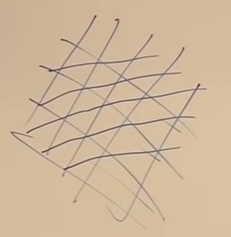
\includegraphics[width=\textwidth]{gr-2-lattice}
	\end{subfigure}
	\begin{subfigure}[t]{0.5\textwidth}
		\caption{Not a Flat Lattice: the bold lines are twice the length of the others, so the central one is forced up, out of blackboard.}\label{fig:gr-2-lattice-not-flat}
		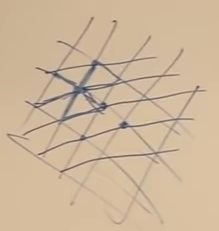
\includegraphics[width=\textwidth]{gr-2-lattice-not-flat}
	\end{subfigure}
\end{figure}

Our problem is to decide whether or not a space is really flat. What are we given? We are given a metric tensor.

\subsection{Transformations}

\subsubsection{Scalars transform trivially}

\begin{align*}
	x^m \leftrightarrow& y^m \\
	S^\prime(y) =& S(x) \text{, we call such an $s$ a scalar}
\end{align*}

\subsubsection{Contravariant \& Covariant Vectors}

Figure \ref{fig:gr-2-coordinates} depicts a coordinate system, and a vector $\vec{V}$.
\begin{figure}[H]
	\caption[A set of coordinates, not necessarily perpendicular.]{A set of coordinates, not necessarily perpendicular (although they could be). Furthermore the distances along the axes are just labels: they need not be equidistant. There are two unit vectors, $\vec{e_1}$ and $\vec{e_2}$ along the $x_1$ and $x_2$ axes.}\label{fig:gr-2-coordinates}
	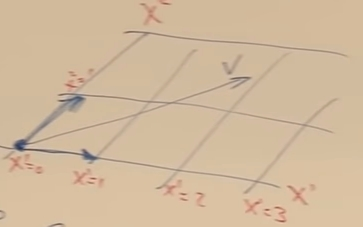
\includegraphics{gr-2-coordinates}
\end{figure}

$\vec{V}$ can be expanded:
\begin{align*}
	\vec{V} =& \sum_i V^i \vec{e_i} \numberthis \label{eq:contravariant:components}
\end{align*}

\begin{defn}[Contravariant components]
	 In (\ref{eq:contravariant:components}), the numbers $V_i$ are called the\emph{ contravariant components} of $\vec{V}$.
\end{defn}

What is $\vec{V} \boldsymbol{\cdot} \vec{e_1}$? If the coordinate system were rectangular, and the labels were equally spaced, it would be $V^1$. As things stand we define:
\begin{align*}
	V_n \triangleq & \vec{V} \boldsymbol{\cdot} \vec{e_n} \numberthis \label{eq:covariant:components}\\
	=& V^m \underbrace{\vec{e_m}\boldsymbol{\cdot} \vec{e_n}}_\text{The metric tensor $g_{mn}$} \numberthis \label{eq:metric_tensor}
\end{align*}

\begin{defn}[Covariant components]
	In (\ref{eq:covariant:components}), the numbers $V^i$ are called the\emph{ covariant components} of $\vec{V}$.
\end{defn}

Let's compute the length of $\vec{V}$.

\begin{align*}
	\vec{V}\boldsymbol{\cdot} \vec{V} =& V^m \vec{e_m}\boldsymbol{\cdot} V^n \vec{e_n}\\
	=& V^m V^n (\vec{e_m}\boldsymbol{\cdot} \vec{e_n})\\
	=&  V^m V^n g_{mn} \text{, where we define $g_{m,n}$ as in (\ref{eq:metric_tensor})}
\end{align*}

If the coordinates are perpendicular, and the separations are the same, the distinction between covariant and contravariant disappears. Polar coordinates are orthogonal, but the separations are not the same.

NB: covariant and contravariant vectors are two different things. Once you introduce a metric tensor it is possible to transform one to the other.

\begin{align*}
	V^{\prime m} =&  \frac{\partial y^m}{\partial x^p} V^p \text{, contravariant transformation}\\
	\frac{\partial S}{\partial y^m} =& \frac{\partial x^p}{\partial y^m} \frac{\partial S}{\partial x^p} \text{, covariant transformation}\\
	W_m^\prime =& \frac{\partial x^p}{\partial y^m} W_p
\end{align*}

I've omitted a discussion of higher rank tensors, which is based on products.

Also if a tensor is zero in one frame it is zero in all frames: if a tensor equation is true in one frame it is true in all frames.

\subsection{Tensor mathematics: addition, multiplication, contraction}

\begin{enumerate}
	\item Addition
	\item Multiplication of Tensors
	\item Contraction
	\item Covariant differentiation
\end{enumerate}

LS presents usual properties, and shows that $g_{mn}$ is a symmetric tensor. He points out that eigenvalues cannot be zero, as otherwise we'd have an elementary vector of zero length. Hence it has an inverse: $g^{mn}g_{np}=\delta_m^p$.


\section{Flatness \& curvature}

''General Relativity has a reputation for being very difficult. I think the reason is because it's very difficult.''--Leonard Susskind

\subsection{Flatness}

A flat geometry is one where all Euclid's postulates are true. It is characterized in terms of the metric: not that $g_{i,j} = \delta_{i,j}$, but rather that coordinates can be found where the metric has such a simple form. More generally, given a metric that is smooth and has all the good differentiable properties, the problem of determining whether or not that space is flat is somewhat difficult. The bad way is to consider all coordinate systems, calculate the metric, and calculate whether it has the required form. The good way is to look for diagnostic quantities, things you can calculate which, if they are zero everywhere the space is flat; if they are non-zero anywhere it means the space is curved there. The diagnostic quantity is called the curvature tensor.

Where want to find a tensor $R$ such that $R=0$ in a flat space.

\begin{align*}
	ds^2 =& g\indices{_{mn}}(x) dx^m dx^n\\
	\exists  g\indices{^{mn}} \mid  g\indices{^{mn}} g\indices{_{nr}} =& \delta\indices{^m_r}\\
	V^m g_{mn} =& V_n\\
	V_m g^{mn} =& V^n
\end{align*}
 
 In Riemannian geometry, unlike Einsteinian, $ds^2 \ge 0$.
 
 \begin{thm}[Gaussian Normal coordinates--Figure \ref{fig:gr-4-gaussian-normal}]
 	At every point, $x_0$ you can choose coordinates such that:
 	\begin{align*}
 	g_{mn}(x_0)=&\delta_{mn}, \text{, and} \numberthis \label{eq:gnf1}\\
 	\frac{\partial g_{m,n}(x_0)}{\partial x^r}=&0 \numberthis \label{eq:gnf2}
 	\end{align*}
 \end{thm}

\begin{figure}[H]
	\begin{center}
		\caption{Gaussian Normal Form}\label{fig:gr-4-gaussian-normal}
		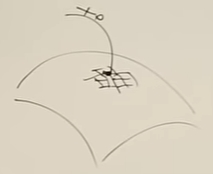
\includegraphics{gr-4-gaussian-normal}
	\end{center}
\end{figure}

\begin{proof}
	Start with some coordinates $y$ and derive new coordinates $x$.
	\begin{align*}
		x^m = y^m + c\indices{^m_{nr}} y^n y^r \text{, assume the same origin.}
	\end{align*}
	In 4 dimensional space there are 40 combinations of $m$, $n$ and $r$; there are 40 coefficients $c\indices{^m_{nr}}$. Moreover (\ref{eq:gnf2}) is actually 40 equations, so we can choose the $c\indices{^m_{nr}}$ so (\ref{eq:gnf2})  is satisfied.
	How do we get the flat metric?
\end{proof}
The problem is that we can't extend away from $x_0$, except in a flat space. The problem is the second derivatives. In general $\frac{\partial^2 g_{m,n}(x_0)}{\partial x^r \partial x^s}\ne0$. The metric is locally flat.

\subsection{Gaussian normal coordinates}

\begin{itemize}
	\item Can we construct a derivative of a tensor?
	\item What does it mean for one vector to be the same as another at a different point? Equality of components isn't enough--Figure \ref{fig:gr-4-equality-of-vectors}. 
\end{itemize}

\begin{figure}[H]
	\begin{center}
		\caption[Comparing vectors at different points]{What does it mean for one vector to be the same as another at a different point? $\frac{\partial V_m}{\partial V^n}=0$ is not a tensor equation, therefore $\frac{\partial V_m}{\partial V^n}$ is not a tensor.}\label{fig:gr-4-equality-of-vectors}
		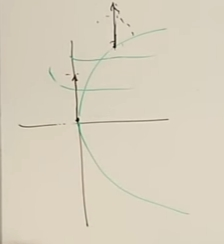
\includegraphics{gr-4-equality-of-vectors}
	\end{center}
\end{figure}

\subsection{Covariant Derivatives}

We need a better definition of the derivative of a vector.

\begin{enumerate}
	\item Create Gaussian normal coordinates.
	\item Pretending that the Gaussian normal coordinates are nice flat coordinates, shift the second vector so its origin is the same as the original vector and the coordinates--Figure \ref{fig:gr-4-equality-of-vectors-revised}.
	\item Take the difference between the two vectors.
	\item Our difference takes into account the change in the vector, and the change in the coordinate system.
\end{enumerate}

\begin{figure}[H]
	\begin{center}
		\caption{Shift the second vector so its origin is the same as the original}\label{fig:gr-4-equality-of-vectors-revised}
		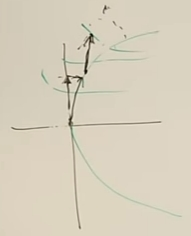
\includegraphics{gr-4-equality-of-vectors-revised}
	\end{center}
\end{figure}

We find:
\begin{align*}
	D_r V_m =& \partial r V_{m} - \Gamma\indices{^t_{rm}} V^t \text{, covariant derivative.} \numberthis \label{eq:covariant_1}\\
	\Gamma\indices{^t_{rm}} =& \Gamma\indices{^t_{rm}}\numberthis \label{eq:symmetry:Gamma}\\
	D_r T_{mn} =& \partial_r T_{mn} - \Gamma\indices{^t_{rm}} T_{tn} - \Gamma\indices{^t_{rn}} T_{mt} \numberthis \label{eq:covariant_2}
\end{align*}

$\Gamma$ is known a "connection", or a Christoffel symbol; which contains various $\frac{\partial g_{m,n}}{\partial x^r}$, which are zero in Gaussian Normal coordinates.

\begin{lemma}[$D_r g_{mn}=0$]\label{thm:covariant_derivative:metric}
	The covariant derivative of the metric tensor is zero.
\end{lemma}

\begin{proof}
	The result follows from the fact that the metric tensor has zero derivatives at $x_0$ in Gaussian Normal coordinates, and the definition of covariant derivative is to differentiate in Gaussian Normal coordinates and treat the result as a tensor.
\end{proof}

\begin{thm}[Christoffel symbols]
	\begin{align*}
		\Gamma\indices{^t_{mn}} =& \frac{1}{2}\big[\partial_n g_{sm} + \partial_m g_{sn}- \partial_s g_{mn}\big]  g^{st}   \numberthis \label{eq:christoffel}
	\end{align*}
\end{thm}

\begin{proof}
	\begin{align*}
		D_s g_{mn} =& \partial_s g_{mn} - \Gamma\indices{^t_{sm}} g_{tn} - \Gamma\indices{^t_{sn}} g_{tm} 	=& 0 \numberthis \label{eq:D:d:1}\\
		D_m g_{sn} =& \partial_m g_{sn} - \underbrace{\Gamma\indices{^t_{sm}}}_\text{From (\ref{eq:symmetry:Gamma})} g_{tn} - \Gamma\indices{^t_{mn}} g_{st} 	=& 0 \numberthis \label{eq:D:d:2}\\
		D_n g_{sm} =& \partial_n g_{sm} - \Gamma\indices{^t_{sn}} g_{tm} - \Gamma\indices{^t_{mn}} g_{st} 	=& 0 \numberthis \label{eq:D:d:3}
	\end{align*}
	
	Now we take (\ref{eq:D:d:3}) + (\ref{eq:D:d:2}) - (\ref{eq:D:d:1}).
	
	\begin{align*}
		\partial_n g_{sm} + \partial_m g_{sn}- \partial_s g_{mn} =& \bcancel{\Gamma\indices{^t_{sn}} g_{tm}} + \Gamma\indices{^t_{mn}} g_{st} + \cancel{\Gamma\indices{^t_{sm}}g_{tn}} + \Gamma\indices{^t_{mn}} g_{st} - \cancel{\Gamma\indices{^t_{sm}} g_{tn}} - \bcancel{\Gamma\indices{^t_{sn}} g_{tm}} \\
		=&2 \Gamma\indices{^t_{mn}} g_{st} \text{, whence}\\
		\Gamma\indices{^t_{mn}} =& \frac{1}{2}\big[\partial_n g_{sm} + \partial_m g_{sn}- \partial_s g_{mn}\big]  g^{st} \numberthis \label{eq:christoffel:g}  
	\end{align*}
\end{proof}

\subsection{The Riemann Curvature Tensor}

We want to define curvature. Consider Figures \ref{fig:gr-4-curved-cone} and \ref{fig:gr-4-curved-cone-vector-field} show that the direction of a vector field changes if we transport it around in a surface that is curved, even though we transported it parallel to itself, i.e. the covariant derivative was zero.
\begin{figure}[H]
	\begin{center}
		\caption{Illustrating curvature}
		\begin{subfigure}[t]{0.4\textwidth}
			\caption{A cone, which is flat everywhere except at the top.}\label{fig:gr-4-curved-cone}
			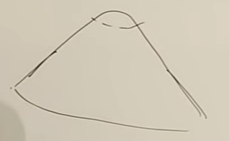
\includegraphics[width=0.9\textwidth]{gr-4-curved-cone}
		\end{subfigure}
		\;
		\begin{subfigure}[t]{0.4\textwidth}
			\caption{Vector field is transported around cone: angle to cut changes!}\label{fig:gr-4-curved-cone-vector-field}
			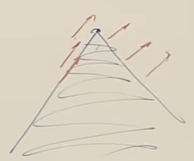
\includegraphics[width=0.9\textwidth]{gr-4-curved-cone-vector-field}
		\end{subfigure}
	\end{center}
\end{figure}

Figure \ref{fig:gr-4-2D} transports a vector along two paths. In a flat space two transported vectors will be identical, $D_r D_s V_m = D_s D_r V_m$, but this is not true in curved space.
\begin{figure}[H]
	\begin{center}
		\caption{Compare vector along two paths}\label{fig:gr-4-2D}
		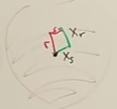
\includegraphics{gr-4-2D}
	\end{center}
\end{figure}

\begin{thm}[Riemann curvature tensor]
	\begin{align*}
		D_s D_r V_m - D_r D_s V_m =& R\indices{_{sr}^t_m} V_t \text{, where the Riemann curvature tensor is}\\
		R\indices{_{sr}^t_m} \triangleq & \partial_r \Gamma \indices{^t_{sm}} - \partial_s \Gamma \indices{^t_{rm}} + \Gamma \indices{^p_{sm}} \Gamma \indices{^t_{pr}}- \Gamma \indices{^p_{rm}} \Gamma \indices{^t_{ps}} 
	\end{align*}
\end{thm}

\begin{proof}
	\begin{align*}
		D_s D_r V_m =& D_s T_{rm} \text{, where}\\
		T_{rm}=& \partial_r V_m -\Gamma \indices{^t_{rm}} V_t \text{, whence}\\
		D_s D_r V_m	=& \partial_s T_{rm} - \Gamma\indices{^t_{sr}} T_{tm} - \Gamma\indices{^t_{sm}} T_{rt} \text{, from (\ref{eq:covariant_2})}\\
		=& \partial_s \big(\partial_r V_m -\Gamma \indices{^t_{rm}} V_t\big) - \Gamma\indices{^t_{sr}} \big(\partial_t V_m -\Gamma \indices{^u_{tm}} V_u\big) - \Gamma\indices{^t_{sm}} \big(\partial_r V_t -\Gamma \indices{^u_{rt}} V_u\big)\\
		=& \partial_s \partial_r V_m - \partial_s \big( \Gamma \indices{^t_{rm}} V_t\big) - \Gamma\indices{^t_{sr}}\partial_t V_m + \Gamma\indices{^t_{sr}} \Gamma \indices{^u_{tm}} V_u - \Gamma\indices{^t_{sm}} \partial_r V_t + \Gamma\indices{^t_{sm}}\Gamma \indices{^u_{rt}} V_u\\
		=& \partial_s \partial_r V_m - \partial_s \big( \Gamma \indices{^t_{rm}} \big)V_t -  \Gamma \indices{^t_{rm}}  \partial_s V_t - \Gamma\indices{^t_{sr}}\partial_t V_m +  \Gamma\indices{^t_{sr}} \Gamma \indices{^u_{tm}} V_u - \Gamma\indices{^t_{sm}} \partial_r V_t + \Gamma\indices{^t_{sm}}\Gamma \indices{^u_{rt}} V_u
	\end{align*}
	
	We interchange the subscripts $r$ and $s$ in the last equation, and then mark the terms that can be cancelled when we subtract, taking into account the symmetry of $g_{rs}$ and $\Gamma\indices{^._{rs}}$.
	
	\begin{align*}
		D_s D_r V_m =&\underbrace{\partial_s \partial_r V_m}_\text{I} - \partial_s \big( \Gamma \indices{^t_{rm}} \big)V_t -  \underbrace{\Gamma \indices{^t_{rm}}  \partial_s V_t}_\text{II} - \underbrace{\Gamma\indices{^t_{sr}}\partial_t V_m}_\text{IV} +  \underbrace{\Gamma\indices{^t_{sr}} \Gamma \indices{^u_{tm}} V_u}_\text{V} - \underbrace{\Gamma\indices{^t_{sm}} \partial_r V_t}_\text{III} + \Gamma\indices{^t_{sm}}\Gamma \indices{^u_{rt}} V_u\\
		D_r D_s V_m =&\underbrace{\partial_r \partial_r V_m}_I - \partial_r \big( \Gamma \indices{^t_{sm}} \big)V_t -  \underbrace{\Gamma \indices{^t_{sm}}  \partial_r V_t}_\text{III} - \underbrace{\Gamma\indices{^t_{rs}}\partial_t V_m}_\text{IV} +  \underbrace{\Gamma\indices{^t_{rs}} \Gamma \indices{^u_{tm}} V_u}_\text{V} - \underbrace{\Gamma\indices{^t_{rm}} \partial_s V_t}_\text{II} + \Gamma\indices{^t_{rm}}\Gamma \indices{^u_{st}} V_u
	\end{align*}
	
	Subtracting, and replacing summation indices in the last two terms, we have:
	\begin{align*}
		D_s D_r V_m - D_r D_s V_m =& \partial_r \big( \Gamma \indices{^t_{sm}} \big)V_t - \partial_s \big( \Gamma \indices{^t_{rm}} \big)V_t + \Gamma\indices{^t_{sm}}\Gamma \indices{^u_{rt}} V_u - \Gamma\indices{^t_{rm}}\Gamma \indices{^u_{st}} V_u\\
		=& \partial_r \big( \Gamma \indices{^t_{sm}} \big)V_t - \partial_s \big( \Gamma \indices{^t_{rm}} \big)V_t + \Gamma\indices{^p_{sm}}\Gamma \indices{^t_{rp}} V_t - \Gamma\indices{^p_{rm}}\Gamma \indices{^t_{sp}} V_t\\
		=& \big[\partial_r  \Gamma \indices{^t_{sm}}  - \partial_s \Gamma \indices{^t_{rm}} + \Gamma\indices{^p_{sm}}\Gamma \indices{^t_{rp}}  - \Gamma\indices{^p_{rm}}\Gamma \indices{^t_{sp}} \big] V_t
	\end{align*}
\end{proof}

The curvature tensor indicates whether or not a space is flat, and it includes the tidal forces.

In Figure \ref{fig:gr-3-move-links} we see the geometric interpretation of {$D_s D_r V_m - D_r D_s V_m$. It measures the stretching that happens when we move the structure of links into the curved region.

\begin{figure}[H]
	\caption[Geometric meaning of $D_s D_r V_m - D_r D_s V_m$]{$D_s D_r V_m - D_r D_s V_m$ measuring the stretching that happens when we move the structure of links into the curved region.}\label{fig:gr-3-move-links}
	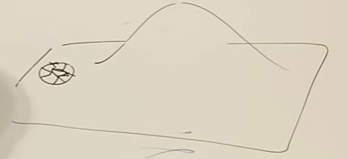
\includegraphics{gr-3-move-links}
\end{figure}


\section{Geodesics \& gravity}

\subsection{Review of Covariant Derivatives}

The point of a covariant derivative is to write a tensor such that in Gaussian Normal Coordinates\footnote{At around this point LS switched to calling Gaussian Normal Coordinates "Perfect Coordinates", but I have retained the original term.} it is just the derivative.

\begin{thm}[Covariant Derivative of contravariant vector]
	\begin{align*}
		D_m V^n =& \partial m V_n + \Gamma\indices{^n_{mr}} V^r
	\end{align*}
\end{thm}

\begin{proof}
	\begin{align*}
		D_m V^n =& D_m\big( g^{np} V_p\big)\\
		=&  \cancel{\big(D_m g^{np}\big) V_p} +  g^{np} D_m V_p \text{,  using Lemma \ref{thm:covariant_derivative:metric}to cancel the first term} \\
		=& g^{np} \big(\partial_m V_p -  \Gamma\indices{^r_{pm}} V_r\big) \text{, from (\ref{eq:covariant_1})}\\
		=& g^{np} \big[\partial_m \big(g_{pq} V^q\big) -  \Gamma\indices{^r_{pm}} g_{rq} V^q\big]\\
		=& g^{np} \big[ \partial_m \big(g_{pq} \big)V^q + g_{pq} \partial_m V^q -  \Gamma\indices{^r_{pm}} g_{rq} V^q\big]\\
		=& \cancel{g^{np} g_{pq}} \partial_m V^q +  g^{np} \big[ \partial_m \big(g_{pq} \big) -   \Gamma\indices{^r_{pm}} g_{rq} \big] V^q \numberthis\label{eq:cov:contra}
	\end{align*}
	Now, using (\ref{eq:christoffel:g})
	\begin{align*}
		 \partial_m g_{pq} -   \Gamma\indices{^r_{pm}} g_{rq} =&\partial_m \big(g_{pq} \big) - \frac{1}{2}\big[\partial_m g_{sp} + \partial_p g_{sm}- \partial_s g_{pm}\big]  \cancel{g^{sr} g_{rq}}\\
		=& \partial_m \big(g_{pq} \big) - \frac{1}{2}\big[\partial_m g_{sp} + \partial_p g_{sm}- \partial_s g_{pm}\big] \partial_m g_{pq} +   \Gamma\indices{^r_{pm}} g_{rq}\\
		 =& \frac{1}{2}\big[\partial_m g_{qp} - \partial_p g_{qm}+ \partial_q g_{pm}\big] 
	\end{align*}
	
	Using (\ref{eq:christoffel:g}) again:
	\begin{align*}
		g^{np} \big[ \partial_m \big(g_{pq} \big) -   \Gamma\indices{^r_{pm}} g_{rq} \big] V^q =& g^{np} \frac{1}{2}\big[\partial_m g_{qp} - \partial_p g_{qm}+ \partial_q g_{pm}\big] V^q\\
		=& \Gamma \indices{^n_{qm}} V^q \text{, and (\ref{eq:cov:contra}) becomes}\\
		D_m V^n =& \partial_m V^n +  \Gamma \indices{^n_{qm}} V^q
	\end{align*}
	
\end{proof}

\subsection{Parallel Transport}

Given a vector field, move along curve. Does vector remain parallel to itself, i.e. $D_m V^n=0$--Figure \ref{fig:gr-4-DV-along-curve}?

\begin{figure}[H]
	\caption{Parallel Transport}
	\begin{center}
		\begin{subfigure}[t]{0.3\textwidth}
			\caption{Transporting vector along curve}\label{fig:gr-4-DV-along-curve}
			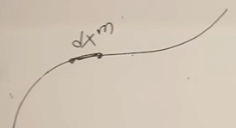
\includegraphics[width=\textwidth]{gr-4-DV-along-curve}
		\end{subfigure}
		\;
		\begin{subfigure}[t]{0.3\textwidth}
			\caption{Parallel Transport is path dependent}\label{fig:gr-4-parallel-transport-path-dependent}
			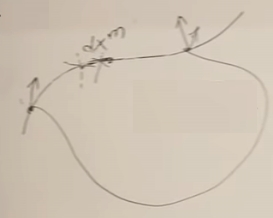
\includegraphics[width=\textwidth]{gr-4-parallel-transport-path-dependent}
		\end{subfigure}
		\;
		\begin{subfigure}[t]{0.3\textwidth}
			\caption{Transporting vectors around a cone gives different results, e.g. the bold portion of the curve versus the rest of the curve. }\label{fig:gr-4-cone-round}
			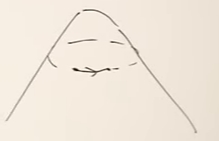
\includegraphics[width=\textwidth]{gr-4-cone-round}
		\end{subfigure}
	\end{center}
\end{figure}

\begin{align*}
	DV^n \triangleq& D_m V^v dx_m\\
	=& \underbrace{\frac{\partial V^n}{\partial x^m} dx^m}_\text{$\triangleq dV^n $} + \Gamma \indices{^n_{mr}} V^r dx^m
\end{align*}

\begin{defn}[Parallel transport]
	If $DV^n=0$ along the curve, we say $V$ is being transported parallel to itself.
\end{defn}

\begin{thm}[Parallel transport preserves length]
	If $DV^n=0$ along the curve, the length of V is preserved.
\end{thm}

\begin{proof}
	The result follows quickly from the following Lemma.
	\begin{lemma}[$D_pV^n=0 \implies \partial_p (g_{mn}V^mV^n)=0$]\label{lemma:d:length}
	\end{lemma}
	\begin{proof}
		\begin{align*}
			\partial_p (g_{mn}V^mV^n)=&\partial_p g_{mn} V^m V^n + g_{mn} \partial_p V^m V^n + g_{mn}V^m  \partial_p V^n\\
			D_pV^n=0 \implies&\partial_p V^n = -\Gamma\indices{^n_{pr}}V^r \text{, so the previous equation becomes:}\\
			\partial_p (g_{mn}V^mV^n)=&\partial_p g_{mn} V^m V^n -g_{mn}\Gamma\indices{^m_{pr}}V^rV^n-\underbrace{g_{mn}\Gamma\indices{^n_{pr}}V^mV^r}_\text{$=g_{nm}\Gamma\indices{^m_{pr}}V^nV^r$}\\
			=&\partial_p g_{mn} V^m V^n -g_{mn}\Gamma\indices{^m_{pr}}V^rV^n-g_{mn}\Gamma\indices{^m_{pr}}V^nV^r \text{, by summetry of $g_{mn}$}\\
			=&\partial_p g_{mn} V^m V^n -2g_{mn}\Gamma\indices{^m_{pr}}V^rV^n \text{, symmetry of $V^rV^n$}\\
			=&\partial_p g_{mn} V^m V^n - g_{mn}\big[\partial_p g_{tr} +\partial_r g_{pt} -\partial_t g_{pr} \big]g^{mt}V^rV^n \text{, from (\ref{eq:christoffel:g})}\\
			=&\partial_p g_{mn} V^m V^n - \underbrace{g_{mn}g^{mt}}_{\delta_n^t}\big[\partial_p g_{tr} +\partial_r g_{pt} -\partial_t g_{pr} \big]V^rV^n
			\\
			=&\partial_p g_{mn} V^m V^n - \big[\partial_p g_{nr} +\partial_r g_{pn} -\partial_n g_{pr} \big]V^rV^n\\
			=&\cancel{\partial_p g_{mn} V^m V^n} - \cancel{\partial_p g_{nr}V^rV^n} -\bcancel{\partial_r g_{pn}V^rV^n} +\bcancel{\partial_n g_{pr} V^rV^n} \text{, on relabelling }\\
			=&0
		\end{align*}
	\end{proof}
	Imagine a curve along which $D_pV^n=0$.  Assume that the length is known at some point, $\vec{x_0}$, on the curve. Then the length at a neighbouring point $\vec{x_0}+\vec{dx}$ is:
	\begin{align*}
		g_{mn}(\vec{x_0}+\vec{dx})V^m(\vec{x_0}+\vec{dx})V^n(\vec{x_0}+\vec{dx})=&	g_{mn}(\vec{x_0})V^m(\vec{x_0})V^n(\vec{x_0})+ \partial_p (g_{mn}V^mV^n) dx^p
	\end{align*}
	But, from Lemma \ref{lemma:d:length}, $\partial_p (g_{mn}V^mV^n)=0$ along the curve, whence:
	\begin{align*}
		g_{mn}(\vec{x_0}+\vec{dx})V^m(\vec{x_0}+\vec{dx})V^n(\vec{x_0}+\vec{dx})=&	g_{mn}(\vec{x_0})V^m(\vec{x_0})V^n(\vec{x_0})
	\end{align*}
\end{proof}

The result of parallel transporting vector in curved space depends on the path--Figures \ref{fig:gr-4-parallel-transport-path-dependent} and \ref{fig:gr-4-cone-round}. 

\begin{figure}[H]
	\begin{center}
		\caption{In general the tangent vector to a curve is not covariantly constant}
		\begin{subfigure}[t]{0.3\textwidth}
			\caption{The cone modified with a sharp point, se we can unroll}\label{fig:gr-4-cone}
			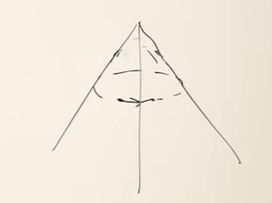
\includegraphics[width=\textwidth]{gr-4-cone}
		\end{subfigure}
		\;
		\begin{subfigure}[t]{0.3\textwidth}
			\caption{Open up the cone and transport a tangent vector, which is changed when it comes back to the original point. The two dots represent the same point.}\label{fig:gr-4-cone-sliced-tangent}
			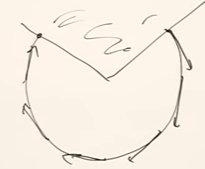
\includegraphics[width=\textwidth]{gr-4-cone-sliced-tangent}
		\end{subfigure}
		\;
		\begin{subfigure}[t]{0.3\textwidth}
			\caption{Add a second vector which maintains the same heading}\label{fig:gr-4-cone-sliced}
			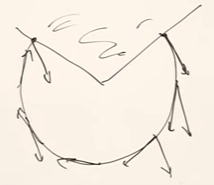
\includegraphics[width=\textwidth]{gr-4-cone-sliced}
		\end{subfigure}
	\end{center}
\end{figure}

 
Figures \ref{fig:gr-4-cone}, \ref{fig:gr-4-cone-sliced-tangent}, and \ref{fig:gr-4-cone-sliced} we slice the cone and open it up. This illustrates the fact that the tangent isn't always parallel to the curve; when it is, the curve is a geodesic, but the curve in Figure \ref{fig:gr-4-cone} is clearly not a geodesic.

\subsection{Geodesics} 

\begin{itemize}
	\item 	A geodesic is a curve whose distance is stationary.
	\item A better definition is to look locally along the curve and require that the curve be as straight as possible.
\end{itemize}

If along the curve the derivative of the tangent vector is zero, that curve is as straight as possible.

In Figure \ref{fig:gr-4-geodesic-intuition} we have a terrain with hills and valleys. We drive a car which is small compared to any curves in the terrain. Point steering wheel to dead straight and start driving without deviating: your path--Figure \ref{fig:gr-4-geodesic-intuition-path}--will be a geodesic.
\begin{figure}[H]
	\begin{center}
		\caption{Intuition for geodesics}
		\begin{subfigure}{0.45\textwidth}
			\caption{Terrain}\label{fig:gr-4-geodesic-intuition}
			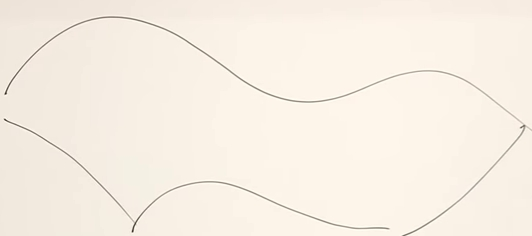
\includegraphics[width=\textwidth]{gr-4-geodesic-intuition}
		\end{subfigure}
		\begin{subfigure}{0.45\textwidth}
			\caption{Your path will be a geodesic}\label{fig:gr-4-geodesic-intuition-path}
			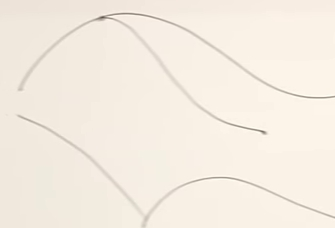
\includegraphics[width=\textwidth]{gr-4-geodesic-intuition-path}
		\end{subfigure}
	\end{center}
\end{figure} 

Figure \ref{fig:gr-4-tangent-vector} illustrates the construction of a unit tangent vector.
\begin{figure}[H]
	\caption[Construction of unit tangent vector]{Construction of unit tangent vector: take the limit as the two points approach each other}\label{fig:gr-4-tangent-vector}
	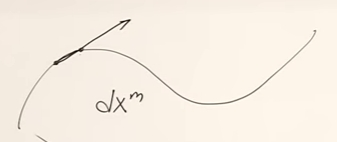
\includegraphics{gr-4-tangent-vector}
\end{figure}

\begin{align*}
	t^m \triangleq& \frac{d x^m}{ds} \text{, we want this to be constant, so}\\
	dt^n + \Gamma \indices{^n_{mr}} t^r dx^m =& 0\\
	\frac{dt^n}{ds}  =& - \Gamma \indices{^n_{mr}} t^r \frac{dx^m}{ds} \\
	=& - \Gamma \indices{^n_{mr}} t^r t^m \text{, or}\\
	\frac{d^2 x^n }{ds^2}=& - \Gamma \indices{^n_{mr}} t^r t^m \text{, equation of motion of a geodesic} \numberthis \label{eq:geodesic}
\end{align*}

So, if $s$ is increasing with time, the left hand side looks like acceleration, and the equation itself looks like Newton's 2nd law. The right hand side depends on the geometry, and the particles moves in the straightest line possible.

So far we have discussed 3 dimensional space, as Riemann knew it. We now move to Minkowskian space-time, with proper time--Figure \ref{fig:gr-4-minkowski-space}

\begin{figure}[H]
	\begin{center}
		\caption{Distance in Minkowski Space}\label{fig:gr-4-minkowski-space}
		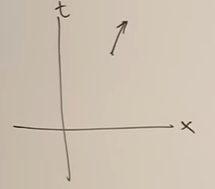
\includegraphics{gr-4-minkowski-space}
	\end{center}
\end{figure}


\begin{align*}
	d \tau^2 =& dt^2 -dx^2 -dy^2 -dz^2\\
	=& - g_{\mu\nu}(x) dx^\mu dx^\nu \text{, where }\\
	g_{\mu\nu} =& \begin{pmatrix}
		-1 &0&0&0\\
		0&1&0&0\\
		0&0&1&0\\
		0&0&0&1
	\end{pmatrix} \numberthis \label{eq:minkowski:metric}\\
	\triangleq& \eta_{\mu\nu} \text{, whence}\\
	d \tau^2=& \eta_{\mu\nu} dx^\mu dx^\nu
\end{align*}

\subsection{Minkowski space}

In 4 dimensions, "flat" means that there is a coordinate system where the metric looks like (\ref{eq:minkowski:metric}).

We want to define a uniformly accelerated motion, but there are problems. \begin{itemize}
	\item If you have a bunch of points which are uniformly separated, \ref{fig:gr-4-uniform-acceleration}, they will maintain a uniform distance, but distances are supposed to transform when they accelerate. If we did this, we'd find the distances getting larger in the rest frame, stretching the strings joining the points, eventually breaking them.
	\item Also the points eventually move faster than the speed of light.
\end{itemize}

\begin{figure}[H]
	\caption[Defining uniform acceleration in Special Relativity]{There is a problem defining uniform acceleration in Special Relativity }\label{fig:gr-4-uniform-acceleration}
	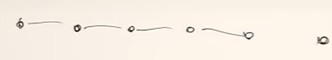
\includegraphics{gr-4-uniform-acceleration}
\end{figure}

We will use an analogue of polar coordinates.

\begin{figure}[H]
	\caption{Constant Acceleration}
	\begin{subfigure}[t]{0.45\textwidth}
		\caption{If the point moves with uniform angular velocity on the circle, the acceleration is uniform, and directed toward the centre.}\label{fig:gr-4-polar}
		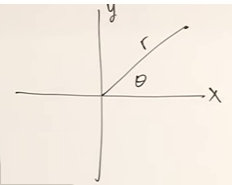
\includegraphics[width=\textwidth]{gr-4-polar}
	\end{subfigure}
	\begin{subfigure}[t]{0.45\textwidth}
		\caption{Constant acceleration in Special Relativity}\label{fig:gr-4-polar-sinh}
		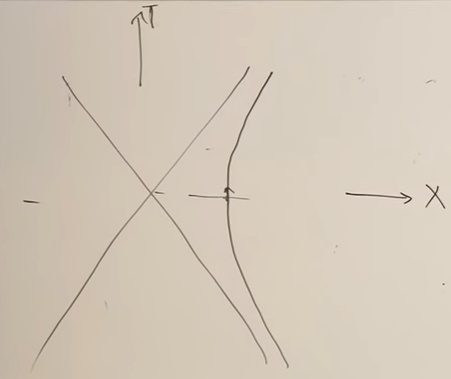
\includegraphics[width=\textwidth]{gr-4-polar-sinh}
	\end{subfigure}
\end{figure}

In Figure \ref{fig:gr-4-polar}
\begin{align*}
	x=& r \cos \theta\\
	y=& r \sin \theta\\
	\cos^2 \theta + \sin^2 \theta =& 1\\
	x^2 + y^2 =& r^2\\
	\cos \theta =& \frac{e^{i \theta}+e^{-i \theta}}{2}\\
	\sin \theta =& \frac{e^{i \theta}-e^{-i \theta}}{2i}
\end{align*}

If the point moves with uniform angular velocity on the circle, the acceleration is uniform, and directed toward the centre.

Figure \ref{fig:gr-4-polar-sinh} depicts constant acceleration in Special Relativity. We replace the trigonometric function by hyperbolic cosines and signs, and the angle $\theta$ is replaces by $\omega$, which increases uniformly. The $\omega$ is like time.

\begin{align*}
	\cosh \omega =& \frac{e^\omega+e^{-\omega}}{2}\\
	\sinh \omega =& \frac{e^\omega-e^{-\omega}}{2}\\
	\cosh^2 \omega +\sinh^2 \omega=& 1\\
	x=& r \cosh \omega\\
	t=& r \sinh \omega\\
	x^2 - t^1 =& 1
\end{align*}

In special relativity $r$ and $\omega$ are the closest thing we have to uniform acceleration--Figure \ref{fig:gr-4-uniform-sinh}. The points along $t=0$ remain the same distance apart as they sweep out their respective hyperbolae.

\begin{figure}[H]
	\begin{center}
		\caption{The closest thing to uniform acceleration in special relativity.}\label{fig:gr-4-uniform-sinh}
		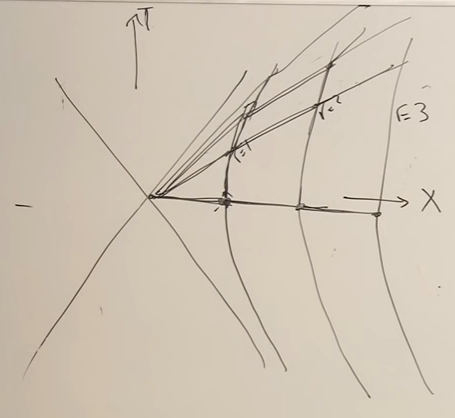
\includegraphics[width=0.8\textwidth]{gr-4-uniform-sinh}
	\end{center}
\end{figure}

Note that the 3 acceleration isn't uniform.

Set:
\begin{align*}
	X=& R \cosh \omega\\
	T=& R \sinh \omega \text{ then the proper acceleration is}\\
	A =& \frac{c^2}{R} \text{, but $c=1$.} \numberthis \label{eq:A:R}
\end{align*}

In hyperbolic polar coordinates
\begin{align*}
	d\tau^2 =& r^2 d \omega^2 - dr^2
\end{align*}

Figure \ref{fig:gr-4-constant-acceleration} depicts constant acceleration.
\begin{figure}[H]
	\begin{center}
		\caption{Constant Acceleration.}
		\begin{subfigure}[t]{0.65\textwidth}
			\caption{Minkowski Space. We go out to a distance R, so acceleration is $g$, then a little further.}\label{fig:gr-4-constant-acceleration}
			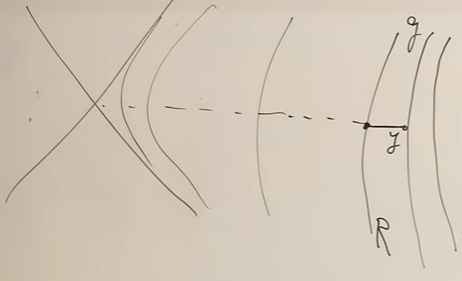
\includegraphics[width=\textwidth]{gr-4-constant-acceleration}
		\end{subfigure}
		\;
		\begin{subfigure}[t]{0.3\textwidth}
			\caption{Little man in elevator with acceleration $g$}\label{fig:gr-4-little-man}
			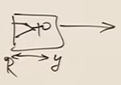
\includegraphics[width=\textwidth]{gr-4-little-man}
		\end{subfigure}
	\end{center}
\end{figure}

At $r=R+y$, the metric is:
\begin{align*}
	d\tau^2 =& \big(R^2 + 2 R y + y^2\big) d \omega^2 - dr^2\\
	=& \big[1 + \frac{2  y}{R} + \big(\frac{y}{R}\big)^2\big] R^2 d \omega^2 - dr^2\\
	=& \big[1 + \frac{2  y}{R} + \big(\frac{y}{R}\big)^2\big] dt^2 - dr^2 \text{, where we define $dt\triangleq R d \omega$}\\
	\approxeq & \big[1 + \frac{2  y}{R} \big] dt^2 - dr^2 \text{, since $y \ll R$. Soopur metric becomes}\\
	d\tau^2 =& \big[1 + 2yg \big] dt^2 - dy^2 \text{, from (\ref{eq:A:R})} \numberthis \label{eq:metric:uniform:acceleration}
\end{align*}

The correction accounts for the gravitational force. We'll see this from the equation of motion. Note that $yg$ is the Newtonian gravitational potential. Figure \ref{fig:gr-4-little-man} depicts the same acceleration being experienced by a little man in an elevator.

Particles move on geodesics of space-time, so they satisfy (\ref{eq:geodesic}).

\begin{align*}
	\frac{d^2 X^n }{d\tau^2}=& - \Gamma \indices{^n_{mr}} t^r t^m \text{, acceleration if velocity $\ll c$}\\
	\frac{d2y}{d\tau^2}=& - \Gamma \indices{^y_{mr}} \frac{dx^r}{d \tau} \frac{dx^m}{d \tau} \text{. Now}\\
	v \ll c \implies & \frac{dx^0}{d \tau} \approxeq 1 \text{ and } \frac{dx^0}{d \tau} \approxeq 0 \text{, so}\\
	\frac{d2y}{d\tau^2}=& - \Gamma \indices{^y_{tt}} \text{, the gravitational force!}\\
	\Gamma\indices{^y_{tt}} =& \frac{1}{2}\big[\underbrace{\partial_n g_{sm} + \partial_m g_{sn}}_\text{$=0$}- \underbrace{\partial_s g_{mn}}_\text{$\frac{\partial g_{tt}}{\partial y}$}\big]  \underbrace{g^{st}}_\text{$g^{yy}=1$} \text{, from (\ref{eq:christoffel})}\\
	\frac{d2y}{d\tau^2}=&\frac{1}{2} \frac{\partial g_{tt}}{\partial y} \text{, derivative potential energy}\\
	=& -g \text{, from (\ref{eq:metric:uniform:acceleration})}
\end{align*}

So we get the same result as Newton's 2nd law. If we had done this calculation in the original frame, where $g_{\mu\nu}=\eta_{\mu\nu}$, we would not have seen the $g$ force. The Christoffel symbols are not tensors! They can be zero in one reference frame, non-zero in another.

We can guess the effect of a real gravitating object--Figure \ref{fig:gr-4-gravitating-object}. We replace the potential energy in (\ref{eq:metric:uniform:acceleration}) with $-\frac{2GM}{y}$

\begin{align*}
	d\tau^2 =& \big[1  -\frac{2GM}{y} \big] dt^2 - dy^2
\end{align*}

Something strange happens when $y-2GM$: $g_{tt}=0$. This has to do with the horizon of a black hole.

\begin{figure}[H]
	\caption{A real gravitating object}\label{fig:gr-4-gravitating-object}
	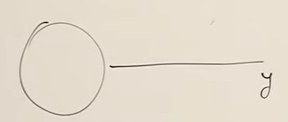
\includegraphics{gr-4-gravitating-object}
\end{figure}



\section{Metric for a gravitational field}

\subsection{Space-like, time-like, and light-like intervals}

In Minkowskian space:
\begin{align*}
	d\tau^2 =dt^2 - \frac{dx^2}{c^2} - \frac{dy^2}{c^2} - \frac{dz^2}{c^2} 
\end{align*}

Sometimes we include c, other times set $c=1$; it depends on whether we want to keep track of how small things are.

\begin{defn}[Timelike]
	If $d\tau^2 >0$ we say the interval is timelike. Figure \ref{fig:gr-5-timelike} illustrates timelike vectors.
\end{defn}

\begin{defn}[Spacelike]
	If $d\tau^2 <0$ we say the interval is spacelike. Spacelike vectors are outside the light cone--Figure \ref{fig:gr-5-timelike}. For a spacelike vector we define $ds^2=-d\tau^2$.
\end{defn}

\begin{defn}[Lightlike]
	If $d\tau^2 =0$ we say the interval is lightlike. These vectors lie in the surface of the lightcone-- Figure \ref{fig:gr-5-timelike}.
\end{defn}

\subsection{Light cone}

\begin{figure}[H]
	\caption{Lightcones}
	\begin{center}
		\begin{subfigure}[t]{0.3\textwidth}
			\caption{SR lightcone, showing timelike vectors.}\label{fig:gr-5-timelike}
			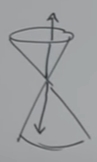
\includegraphics{gr-5-timelike}
		\end{subfigure}
		\;
		\begin{subfigure}[t]{0.65\textwidth}
			\caption{A selection of tipped and tilty lightcones, typical of GR. Shape of lightcone varies as we move around space.}\label{fig:gr-5-tipped-tilty-lightcone}
			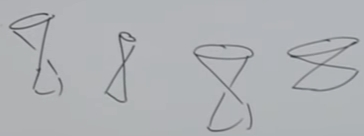
\includegraphics[width=\textwidth]{gr-5-tipped-tilty-lightcone}
		\end{subfigure}
	\end{center}
\end{figure}

\begin{itemize}
	\item The proper time is the time read off by a clock moving along a timelike trajectory;
	\item proper distance is the distance measured bt a metre stick along a spacelike trajectory.
\end{itemize} 

In general $g_{\mu\nu}$ is a function of position in space time, $g_{\mu\nu}(x)$. It cannot be just any old function: it must be a matrix with one negative eigenvalue (time) and 3 positive. We must have time everywhere, and a there is a lightcone everywhere. Figure \ref{fig:gr-5-tipped-tilty-lightcone} shows a selection of tipped and tilty lightcones, which reflects the fact that the coordinates might be curvy and wavy. At every point there is a notion of timelike vectors inside the cone, and spacelike outside. Phones move on the surface of the lightcone.

\begin{defn}[Signature]
	The collection of signs of the eigenvalues is known as the signature. The signature of Minkowski space is $\{-,+,+,+\}$. We must be sure that our metric has the correct signature.
\end{defn}

Any timelike vector is an eigenvector with eigenvalue -1; any spacelike vector is an eigenvector, eigenvalue +1;

We return to geodesics. Consider the proper time interval between two points. We will treat this as \emph{action} (actually $Action=-m\tau$), and find the path that gives stationary action, using the Euler Lagrange Equations\cite{susskind2013quantum}.

\begin{align*}
	\tau =& \int_{1}^{2} \sqrt{-g_{\mu\nu}(x) dx^\mu dx^\nu } \\
	S =& -m \int_{1}^{2} \underbrace{\sqrt{-g_{\mu\nu}(x) \frac{dx^\mu}{dt} \frac{dx^\nu}{dt} }}_\text{$=\Lagr(x,\dot{x})$--Lagrangian}  dt \numberthis \label{eq:action:g}\\
	=& -m \int_{1}^{2} \Lagr(x,\dot{x}) dt
\end{align*}

 N.B. $-g_{\mu\nu}(x) dx^\mu dx^\nu>0$ along a timelike path. The action is minimized if we move along a path that satisfies the Euler-Lagrange equations.
 
\begin{align*}
 	\frac{d}{dt}\big(\frac{\partial \Lagr}{\partial \dot{x}}\big) =& \frac{\partial \Lagr}{\partial x} \numberthis \label{eq:euler:lagrange}
\end{align*}

\begin{thm}[Euler Lagrange equation and geodesic]
	If the action is defined by (\ref{eq:action:g}), the Euler Lagrange equation (\ref{eq:euler:lagrange}) is equivalent to the geodesic equation (\ref{eq:geodesic}).
\end{thm}
\begin{proof}
	From (\ref{eq:action:g}):
	\begin{align*}
		\Lagr =& \sqrt{-g_{\mu\nu} \dot{x}^\mu \dot{x}^\nu} \text{, so}\\
		\frac{d}{d\tau}\big(\frac{\partial \Lagr}{\partial \dot{x}^\rho}\big) =& \frac{d}{d\tau} \big( \frac{-\frac{\cancel{2}}{\cancel{2}}g_{\rho\nu}  \dot{x}^\nu}{\underbrace{\sqrt{-g_{\mu\nu} \dot{x}^\mu \dot{x}^\nu}}_\text{$=1$, since $d\tau^2=-g_{\mu\nu}dx^\mu dx^\nu$}}\big)\\
		=&-\frac{d}{d\tau}\big[g_{\rho\nu}  \dot{x}^\nu\big]\\
		=&- \partial_\sigma g_{\rho\nu}  \dot{x}^\nu \dot{x}^\sigma- g_{\rho\nu} \ddot{x}^\nu 
	\end{align*}
	
	\begin{align*}
		\frac{\partial \Lagr}{\partial x^\rho}=& \frac{-\frac{1}{2}{\partial_\rho g_{\mu\nu}} \dot{x}^\mu \dot{x}^\nu}{\underbrace{\sqrt{-g_{\mu\nu} \dot{x}^\mu \dot{x}^\nu}}_\text{$=1$, similarly}} 
	\end{align*}
	so the Euler Lagrange equations become
	\begin{align*}
		 g_{\rho\nu} \ddot{x}^\nu =& \frac{1}{2} \partial_\rho g_{\mu\nu} \dot{x}^\mu \dot{x}^\nu - \partial_\sigma g_{\rho\nu}  \dot{x}^\nu \dot{x}^\sigma\\
		 =& \frac{1}{2} \partial_\rho g_{\mu\nu} \dot{x}^\mu \dot{x}^\nu - \frac{1}{2}\partial_\sigma g_{\rho\nu}  \dot{x}^\nu \dot{x}^\sigma - \frac{1}{2}\partial_\sigma g_{\rho\nu}  \dot{x}^\nu \dot{x}^\sigma\\
		 =& \frac{1}{2} \partial_\rho g_{\mu\nu} \dot{x}^\mu \dot{x}^\nu - \frac{1}{2}\partial_\nu g_{\rho\mu}  \dot{x}^\mu \dot{x}^\nu - \frac{1}{2}\partial_\mu g_{\rho\nu}  \dot{x}^\nu \dot{x}^\mu\\
		 =& \frac{1}{2} \big[ \partial_\rho g_{\mu\nu} - \partial_\nu g_{\rho\mu}  - \partial_\mu g_{\rho\nu} \big]  \dot{x}^\mu \dot{x}^\nu \\
		g^{\sigma\rho} g_{\rho\nu} \ddot{x}^\nu =&\frac{1}{2}g^{\sigma\rho} \big[ \partial_\rho g_{\mu\nu} - \partial_\nu g_{\rho\mu}  - \partial_\mu g_{\nu\rho} \big]  \dot{x}^\mu \dot{x}^\nu\\
		\ddot{x}^\sigma =& - \Gamma\indices{^\sigma_{\mu\nu}}\dot{x}^\mu \dot{x}^\nu \text{, which matches (\ref{eq:geodesic})}
	\end{align*}
\end{proof}

\subsection{Schwarzschild metric}

We start with the following metric.

\begin{align*}
	d \tau^2 =& \bigg(1+\frac{2 U(x)}{c^2}\bigg) dt^2 - \frac{1}{c^2} ds^2 \text{, where U(x) is the gravitational potential} \numberthis \label{eq:sch:ansatz}\\
	S =& -m c^2 \int_{1}^{2} \sqrt{\bigg(1+\frac{2U}{c^2}\bigg) - \frac{1}{c^2}\dot{X}^2} dt\\
	=& -m c^2 \int_{1}^{2} \sqrt{1 +\frac{1}{c^2}\big(2U-\dot{X}^2\big)} dt\\
	\approxeq& -m c^2 \int_{1}^{2} \big[1 + \frac{1}{2c^2}\big(2U-\dot{X}^2\big)\big] \text{, if velocity small (Binomial Theorem)}\\
	=& -m c^2 -mU + \frac{m}{2} \dot{X}^2 \text{, plugging into Euler-Largange we get}\\
	m\ddot{X} =& -m \nabla U \text{, Newton's second law.}
\end{align*}

We learn from this that the $g_00$ term in (\ref{eq:sch:ansatz}) gives riser to Newton's 2nd law for motion in a gravitational field for small velocity.

Consider the gravitational field of the Sun.

\begin{align*}
	U(X) =& - \frac{MG}{r(X)} \text{, and adopt the \emph{ansatz}}\\
		d \tau^2 =& \bigg(1-\frac{2 MG}{c^2 r}\bigg) dt^2 - \frac{1}{c^2} \big(dx^2 + dy^2 +dz^2\big) \text{. Now}\\
		dx^2 + dy^2 +dz^2 =& dr^2 + r^2 \big(\underbrace{d\theta^2 + cos^2 \theta d\phi^2}_\text{$\triangleq d\Omega^2$}\big) \text{, whence}\\
		d \tau^2 =& \bigg(1-\frac{2 MG}{c^2 r}\bigg) dt^2 - \frac{1}{c^2}dr^2 - \frac{1}{c^2} r^2 d\Omega^2
\end{align*}

Now there is a problem with $\bigg(1-\frac{2 MG}{c^2 r}\bigg)$ when r is too small; $g_00$ becomes negative, which gives a signature that is not physical.

\begin{align*}
	\bigg(1-\frac{2 MG}{c^2 r}\bigg) = \frac{r-\underbrace{\frac{2 MG}{c^2}}_\text{Schwartzchild radius}}{r}
\end{align*}

When $r$ is less that the Schwartzchild radius, we have crossed into a region with 4 space dimensions and no time dimensions, which is bad. We need a coefficient for $r^2$, so it turns into a time dimension when $t$ turns into space. We will see later that this works.

\begin{align*}
	d \tau^2 =& \bigg(1-\frac{2 MG}{c^2 r}\bigg) dt^2 - \frac{dr^2}{\bigg(1-\frac{2 MG}{c^2 r}\bigg)c^2} - \frac{1}{c^2} r^2 d\Omega^2 \numberthis \label{eq:schwartzchild}
\end{align*}

\subsection{Black holes and the Event horizon}

We want to see how relativistic particles move in this metric. We choose units where $c=1$, and consider two types of orbits, radial and circular. In Figure \ref{fig:gr-5-falling-in}  The external observer uses time $t$, and the person falling in uses $\tau$.

\begin{figure}[H]
	\caption[Falling into black hole]{Falling into black hole. The external observer uses $t$, and the person falling in uses $\tau$.}\label{fig:gr-5-falling-in}
	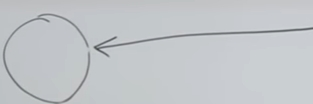
\includegraphics{gr-5-falling-in}	
\end{figure}

\begin{align*}
d \tau^2 =& \bigg(1-\frac{2 MG}{ r}\bigg) dt^2 - \frac{dr^2}{\bigg(1-\frac{2 MG}{ r}\bigg)} - \underbrace{ r^2 d\Omega^2}_\text{, assume angle doesn't change}\\
S =& -m \int \sqrt{\big(1-\frac{2 MG}{ r}\big)  - \frac{\dot{r}^2}{\big(1-\frac{2 MG}{ r}\big)}} dt\\
\Lagr  =& -m \sqrt{\big(1-\frac{2 MG}{ r}\big)  - \frac{\dot{r}^2}{\big(1-\frac{2 MG}{ r}\big)}} 
\end{align*}
Now Energy should be conserved: we can get this from the Hamiltonian.

\begin{align*}
	P_r =& \frac{\partial \Lagr}{\partial r}\\
	P_r \dot{r} - \Lagr =& H\\
	H =& \frac{\big(1-\frac{2MG}{r}\big)m}{\sqrt{\big(1-\frac{2 MG}{ r}\big)  - \frac{\dot{r}^2}{\big(1-\frac{2 MG}{ r}\big)}}}\\
	=& E \text{, constant. Whence}\\
	\dot{r}^2 =& \big(1-\frac{2MG}{r}\big)^2- \frac{\big(1-\frac{2MG}{r}\big)^3}{E^2}\\
	\dot{r} \approx & \sqrt{\frac{r-2MG}{MG}} \text{ near the event horizon.}
\end{align*}
The particles slows down asymptotically as it approaches the event horizon, and never actually gets there!

Consider a light ray, Figure \ref{fig:gr-5-lightray}, which moves along the surface of the light cone.
 
\begin{figure}[H]
	\caption{Light Ray on surface of light cone.}\label{fig:gr-5-lightray}
	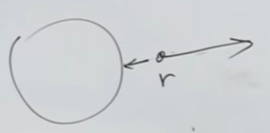
\includegraphics{gr-5-lightray}
\end{figure}

\begin{align*}
	d \tau^2 =& \bigg(1-\frac{2 MG}{ r}\bigg) dt^2 - \frac{dr^2}{\bigg(1-\frac{2 MG}{ r}\bigg)}\\
	=& 0 \text{, on the light cone, i.e.}\\
	\bigg(1-\frac{2 MG}{ r}\bigg)^2 dt^2 =& dr^2\\
	\dot{r} =& \pm \frac{r-2MG}{r}
\end{align*}

So the speed of light is zero at the event horizon!


\section{Black holes}


The Schwarzschild solution is an idealization. $F = \frac{mMg}{r^2}$ is itself an idealization, based on the assumption that the mass $M$ is concentrated at a point. For a realistic mass this isn't return inside the object. For a real mass if you squeeze everything to be arbitrarily small it will spring back. This isn't so in the General Theory of Relativity. Figure \ref{fig:gr-6-centrifugal-force} illustrates the fact that in Newtonian mechanics an incoming particle is infinitely unlikely to hit a point mass, despite the very strong gravitational attraction. This isn't true in General Relativity; the black hole pulls anything into the centre..

\begin{figure}[H]
	\caption[Centrifugal force]{In Newtonian physics, a particle heading for a massive particle will hit it only if it is aimed with absolute precision. Otherwise centrifugal force will cause it so swing past..}\label{fig:gr-6-centrifugal-force}
	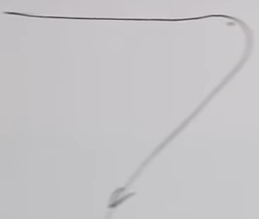
\includegraphics{gr-6-centrifugal-force}
\end{figure} 

\subsection{Schwarzschild metric}

From (\ref{eq:schwartzchild}), the Schwarzschild metric is:
\begin{align*}
	d \tau^2 =&\bigg(1-\frac{2MG}{r}\bigg)dt^2-\frac{dr^2}{1-\frac{2MG}{r}} - r^2 d\Omega^2 
\end{align*}

Notice that $1-\frac{2MG}{r}$ changes sign when $r=2MG$, but the signature of the metric is unchanged, even though the signs of $dt$ and $dr$ change. See Figure \ref{fig:gr-6-schwartzchild-radius}. The metric also blows up when $r\rightarrow0$. We shall see that the first problem isn't serious, but the 2nd is.

\subsection{Schwarzschild Radius/Black hole event horizon}

\begin{figure}[H]
	\begin{center}
		\caption[Illustrating the Schwarzschild Metric]{Illustrating the Schwarzschild Metric. The vertical axis represents time.}
		\begin{subfigure}[t]{0.45\textwidth}
			\caption{Far away (large $r$) this behaves like flat space: $ d \tau^2 =dt^2-dr^2 - r^2 d\Omega^2$. Notice that something funny happens at $r=2MG$: this is known as the Schwarzschild radius, and the Event Horizon.}\label{fig:gr-6-schwartzchild-radius}
			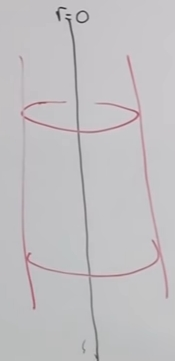
\includegraphics[width=\textwidth]{gr-6-schwartzchild-radius}
		\end{subfigure}
		\begin{subfigure}[t]{0.45\textwidth}
			\caption{A metre stick falls in. As we saw earlier, it slows down and approaches the Event Horizon asymptotically. As the metre stick falls, the two ends approach each other: this is, in fact, a Lorentz transformation.}\label{fig:gr-6-infalling}
			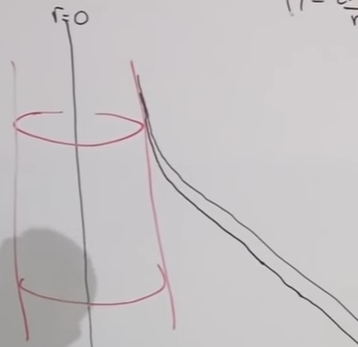
\includegraphics[width=\textwidth]{gr-6-infalling}
		\end{subfigure}
	\end{center}
\end{figure}

Figure \ref{fig:gr-6-infalling} depicts a metre stick falling towards the event horizon. Imagine that the mere stick is also a clock, which will measure proper time $d\tau$, not coordinate time $dt$. When it is very far away, $r\approxeq\infty$, $d\tau\approxeq dt$. As it approaches we get less and less $\tau$ for $t$; we will see that there is only a finite $\tau$ elapsed to reach the Event Horizon, despite requiring an infinite $t$.


\subsection{Light ray orbiting a black hole}

Consider a beam of light passing outside the event horizon and being bent by the gravitational field--Figure \ref{fig:gr-6-bent-light-ray}. If the field is strong enough it will be bent into a circle.
\begin{figure}[H]
	\caption{Light ray being bent my massive object}
	\begin{subfigure}[t]{0.45\textwidth}
		\caption{Bent light ray}\label{fig:gr-6-bent-light-ray}
		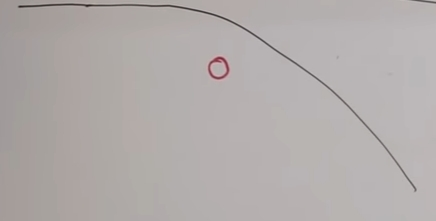
\includegraphics[width=\textwidth]{gr-6-bent-light-ray}
	\end{subfigure}
	\begin{subfigure}[t]{0.45\textwidth}
		\caption{Circular orbit}\label{fig:gr-6-circular-trajectory}
		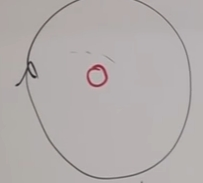
\includegraphics[width=\textwidth]{gr-6-circular-trajectory}
	\end{subfigure}
\end{figure}

\begin{thm}[Photosphere]
	There is an unstable orbit for a light beam at $r=3MG$.
\end{thm}

\begin{proof}
	The argument is essentially classical, except for the use of the Schwarzschild metric to define the action:
	\begin{enumerate}
		\item construct Lagrangian $\Lagr$;
		\item use conservation laws for a particle of mass $m$;
		\item calculate energy as a function of $r$;
		\item determine extremum of energy;
		\item let $m\rightarrow0$.
	\end{enumerate}
	
	The action is given by:
	
	\begin{align*}
		S =&-m \int d\tau\\
		=& -m \int \sqrt{\underbrace{\bigg(1-\frac{2MG}{r}\bigg)}_\text{$=\mathscr{F}$, say}dt^2-\underbrace{\frac{1}{1-\frac{2MG}{r}}}_\text{$=\mathscr{G}$, say}dr^2 - r^2 d\Omega^2} \\
		=& -m \int \sqrt{\mathscr{F}(r)-\mathscr{G}(r)\dot{r}^2 - r^2 \dot{\theta}^2} dt \text{, where $\theta$ has been chosen suitably.}\\
		\Lagr =& -m \sqrt{\mathscr{F}(r)-\mathscr{G}(r)\dot{r}^2 - r^2 \dot{\theta}^2} \text{ is the Lagrangian.}
	\end{align*}
	
	Now there are two conservation laws, energy and angular momentum. We calculate the two momenta, angular and radial.
	\begin{align*}
		L =& P_{\theta} \text{, angular momentum}\\
		=& \frac{\partial \Lagr}{\partial \dot{\theta}}\\
		=& \frac{m r^2 \dot{\theta}}{\sqrt{\mathscr{F}(r)-\mathscr{G}(r)\dot{r}^2 - r^2 \dot{\theta}^2}} \text{, constant.} \numberthis \label{eq:L:light:orbit}\\
		=& m \Lambda \text{, where $\Lambda\triangleq\frac{r^2 \dot{\theta}}{\sqrt{\mathscr{F}(r)-\mathscr{G}(r)\dot{r}^2 - r^2 \dot{\theta}^2}}$, is also conserved}\\
		P_r =& \frac{\partial \Lagr}{\partial \dot{r}}\\
		=& \frac{m \mathscr{G} \dot{r}}{\sqrt{\mathscr{F}(r)-\mathscr{G}(r)\dot{r}^2 - r^2 \dot{\theta}^2}}
	\end{align*}
	
	$P_r$ is not conserved, but the energy is. The energy is given by the classical Hamiltonian.
	\begin{align*}
		H =& P_r \dot{r} + L \dot{\theta} - \Lagr\\
		=& \frac{m \mathscr{G} \dot{r}}{\sqrt{\mathscr{F}(r)-\mathscr{G}(r)\dot{r}^2 - r^2 \dot{\theta}^2}}\dot{r} + \frac{m r^2 \dot{\theta}}{\sqrt{\mathscr{F}(r)-\mathscr{G}(r)\dot{r}^2 - r^2 \dot{\theta}^2}}\dot{\theta}  +m \frac{\mathscr{F}(r)-\mathscr{G}(r)\dot{r}^2 - r^2 \dot{\theta}^2}{\sqrt{\mathscr{F}(r)-\mathscr{G}(r)\dot{r}^2 - r^2 \dot{\theta}^2}}\\
		=& \frac{\cancel{m \mathscr{G} \dot{r}^2} + \bcancel{m r^2\dot{\theta}^2} + m\mathscr{F}(r)-\cancel{m\mathscr{G}(r)\dot{r}^2} - \bcancel{mr^2 \dot{\theta}^2} }{\sqrt{\mathscr{F}(r)-\mathscr{G}(r)\dot{r}^2 - r^2 \dot{\theta}^2}}\\
		=& \frac{\mathscr{F}(r)m}{\sqrt{\mathscr{F}(r)-\mathscr{G}(r)\dot{r}^2 - r^2 \dot{\theta}^2}} \\
		=& E \text{. So, for a circular orbit}\\
		E =& \frac{\mathscr{F}(r)m}{\sqrt{\mathscr{F}(r)- r^2 \dot{\theta}^2}} \text{. Now from (\ref{eq:L:light:orbit})}\\
		\frac{L}{M} =& \frac{r^2 \dot{\theta}}{\sqrt{\mathscr{F}(r) - r^2 \dot{\theta}^2}}\\
		=& \Lambda \text{, reduced angular momentum}
	\end{align*}
	
	Solving for $\dot{\theta}$:
	\begin{align*}
		\Lambda^2 =& \frac{r^4 \dot{\theta}^2}{\mathscr{F}(r) - r^2 \dot{\theta}^2}\\
		\Lambda^2 \big(\mathscr{F}(r) - r^2 \dot{\theta}^2\big)	=& r^4 \dot{\theta}^2\\
		\Lambda^2 \mathscr{F}(r) =& \Lambda^2 r^2 \dot{\theta}^2 +  r^4 \dot{\theta}^2\\
		=& \big(\Lambda^2 r^2  +  r^4\big) \dot{\theta}^2\\
		\dot{\theta}^2=& \frac{\Lambda^2 \mathscr{F}(r)}{\Lambda^2 r^2  +  r^4}
	\end{align*}
	
	Substituting in (\ref{eq:L:light:orbit}):
	\begin{align*}
		E =& \frac{\mathscr{F}(r)m}{\sqrt{\mathscr{F}(r)- r^2 \dot{\theta}^2}}\\
		=&  \frac{\mathscr{F}(r)m}{\sqrt{\mathscr{F}(r)- r^2 \frac{\Lambda^2 \mathscr{F}(r)}{\Lambda^2 r^2  +  r^4}}}\\
		E^2=&  \frac{\mathscr{F}(r) \bcancel{\mathscr{F}(r)}m^2 \big(\Lambda^2 r^2  +  r^4\big)}{\bcancel{\mathscr{F}(r)}\big(\cancel{\Lambda^2 r^2}  +  r^4\big)- \cancel{r^2 \Lambda^2 \mathscr{F}(r)}} \text{, whence:}\\
		E =& \frac{\sqrt{\mathscr{F}} \sqrt{r^2 \Lambda^2 + r^4}}{r^2} m
	\end{align*}
	
	We want now to let $m \rightarrow 0$ for a photon. We want to minimize the energy for a fixed $\Lambda$. As $m \rightarrow 0$, for fixed $L$, $\Lambda\rightarrow\infty$, whence $\sqrt{r^2 \Lambda^2 + r^4} m \rightarrow \sqrt{r^2 \Lambda^2 } m \rightarrow rL$. In the limit:
	\begin{align*}
		E =& \frac{\sqrt{\mathscr{F}} L }{r}
	\end{align*}
	Equilibrium is when this is minimized/maximized--Figure \ref{fig:gr-6-energy-r}
	\begin{align*}
		E 		=& \frac{\sqrt{1-\frac{2MG}{r}} L }{r}\\
		\log{E} =& \frac{1}{2} \log{(1-\frac{2MG}{r})} - \log{r}\\
		\frac{1}{E} \frac{dE}{dr} =& \frac{1}{\cancel{2}} \frac{\cancel{2}MG}{r^2 (1-\frac{2MG}{r})} - \frac{1}{r}\\
		=& \frac{MG}{r(r-2MG)} -\frac{(r-2MG)}{r(r-2MG)}\\
		=& \frac{3MG-r}{r(r-2MG)}\\
		=& 0 \iff r=3MG
	\end{align*}	
	Figure \ref{fig:gr-6-energy-r} shows an unstable equilibrium at $r=3MG$.
	
	\begin{defn}[photon-sphere/photo-sphere]
		This sphere of radius $3MG$ is called the photon-sphere or photo-sphere. It does not depend on $L$!.
	\end{defn} 

	 If a photon comes in and is slightly outside photon-sphere it can whip around black hole multiple times before going out. If it is slightly inward it will spiral into horizon. (A massive particle inside photon-sphere will also fall in.)

\end{proof}	
	
\begin{figure}[H]
	\begin{center}
		\caption[Energy near black hole horizon]{Energy near black hole horizon: $E=\frac{\sqrt{1-\frac{2MG}{r}}  }{r}L$. At $r=2MG$, E=0. As $r \rightarrow \infty$, E behaves like a straight line. As $r \rightarrow \infty$ E behaves like $\frac{1}{r}$. There should be a maximum in between. }\label{fig:gr-6-energy-r}
		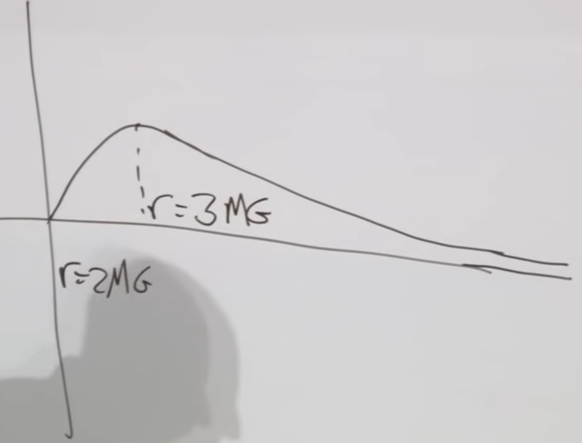
\includegraphics{gr-6-energy-r}
	\end{center}
\end{figure}


\begin{table}
	\caption{Behaviour of orbit near photosphere}
	\begin{center}
		\begin{tabular}{|c|c|c|} \hline
			&Photon&Massive\\ \hline
			$r<3MG$&Spirals in&Spirals in\\ \hline
			$r=3MG$&Unstable equilibrium&\\ \hline
			$r>3MG$&Spirals out&May have stable orbit\\\hline
		\end{tabular}
	\end{center}
\end{table}

\begin{figure}[H]
	\caption[Light beams going past Black Hole]{Light beams going past Black Hole. Top light beam is bent, so it appears to be coming from further out. Object behind Black Hole heas its beams bent, but they converge at the eye; they become a ring. Finally light ray from back, near black hole, is also bent so it can be seen. }\label{fig:gr-6-light-rays-black-hole}
	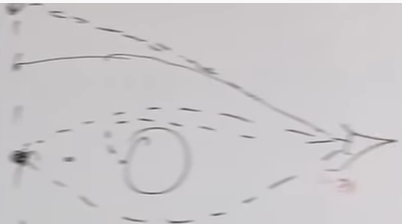
\includegraphics{gr-6-light-rays-black-hole}
\end{figure}


\subsection{Hyperbolic coordinates}

Many things that happen in gravity an be understood via an uniformly accelerated coordinate system. Gravity is often not the same thing as a uniformly accelerated coordinate system, but the uniformly accelerated coordinate system is often useful in understanding gravity--Figure \ref{fig:gr-6-hyperbolic-coordinates}.

\begin{figure}[H]
	\caption[Hyperbolic coordinates. ]{Hyperbolic coordinates. Each dotted hyperbola is a surface on which $	X^2 - T^2 = constant$, and represents constant acceleration.}\label{fig:gr-6-hyperbolic-coordinates}
	\includegraphics{gr-6-hyperbolic-coordinates}
\end{figure}

\begin{align*}
	X =& \rho \cosh{\omega} \\
	T =& \rho \sinh{\omega}\\
	X^2 - T^2 =& 1 \text{. The metric is given by:}\\
	d\tau^2 =& \rho^2 d\omega^2 - d \rho^2 
\end{align*}

We introduce new coordinates:
\begin{align*}
	\rho^2 =& 4 \xi\\
	\omega =& \frac{t}{2} \text{ and the metric becomes}\\
	d\tau^2 =& \xi dt^2 - \frac{d \xi^2}{\xi} \numberthis \label{eq:tau:xi}
\end{align*}

This is a bit like the Schwarzschild metric (\ref{eq:schwartzchild}). We will consider the case where $r \approxeq \frac{2MG}{r}$.

\begin{align*}
	\frac{r-2MG}{r} \approxeq & \frac{r-2MG}{2MG}\\
	d \tau^2 =& \frac{r-2MG}{2MG} dt^2 - \frac{2MG}{r-2MG}dr^2
\end{align*}

Now use the Schwarzschild radius as the unit of length.

\begin{align*}
	d \tau^2 =& (r-1) dt^2 - \frac{1}{r-1}dr^2\\ \text{, now call $r-1$ $\xi$}\\
	d \tau^2 =& \xi dt^2 - \frac{1}{\xi} d\xi^2 \text{, which matches(\ref{eq:tau:xi}) }
\end{align*}

This tells us that the vicinity of the horizon is locally flat, since we can transform the singularity away. 

What about the business of time becoming space and vice versa? Since $\xi=r-1$, it changes sign as we cross the event horizon. What does it mean in the flat space? We have $\rho^2 = 4 \xi$. How can it be negative? Think instead of $X^2-T^2=\rho^2$. Positive values represent the hyperbolae in - Figure \ref{fig:gr-6-hyperbolic-coordinates}: $\lvert X\rvert>\lvert T\rvert$ in the whole quadrant. If $\rho^2$, $\lvert X\rvert<\lvert T\rvert$ corresponds to the top quadrant. Figure \ref{fig:gr-6-cross-event-horizon} depicts an object crossing the event horizon. A spacelike coordinate $\xi$ has become timelike. What happens to $\omega$? Figure \ref{fig:gr-6-cross-event-horizon-omega} depicts a spacelike hyperbola becoming timelike (coordinates can do whatever they want to: physics limits physical objects only).

\begin{figure}[H]
	\caption{Crossing the event horizon}
	\begin{subfigure}[t]{0.3\textwidth}
		\caption{Point comes in with $\omega=0$ and crosses event horizon.}\label{fig:gr-6-cross-event-horizon}
		\includegraphics[width=\textwidth]{gr-6-cross-event-horizon}
	\end{subfigure}
	\begin{subfigure}[t]{0.3\textwidth}
		\caption{Point comes in with $\omega=0$ and crosses event horizon.}\label{fig:gr-6-cross-event-horizon-omega}
		\includegraphics[width=\textwidth]{gr-6-cross-event-horizon-omega}
	\end{subfigure}
	\begin{subfigure}[t]{0.3\textwidth}
		\caption{The singularity is not a place; it's a time} \label{fig:gr-6-singularity}
		\includegraphics[width=\textwidth]{gr-6-singularity}
	\end{subfigure}
\end{figure}

So all that happens is $(\xi,\omega)$ interchange their roles. The same thing is true of the Schwarzschild coordinates. In Figure \ref{fig:gr-6-cross-event-horizon-omega}, as we decrease $r$ past the event horizon we follow the arrows, and turn up at the event horizon. We continue until $r=0$: then something nasty happens.

\subsection{Black hole singularity}

In Figure \ref{fig:gr-6-singularity} we see that the singularity is not a place; it's a time. The surface $r=0$ is spacelike, not timelike. You can't avoid it, because you can't avoid the future. If you are inside the event horizon, the singularity is in your future.

We want to understand the discrepancy between the  time as perceived by an object falling  into a black hole, and the observer who is left behind. Figure \ref{fig:gr-6-alice-bob} depicts Alice throwing Bob into the Black Hole. Alice never sees Bob go throw the horizon, as this requires infinite $\omega$, hence infinite $t$. Bob just ticks off time and crosses the event horizon. Alice sees Bob slowed down: each heartbeat of Bob takes longer and longer. What does Bob see? Figure \ref{fig:gr-6-bobs-perspective} depicts the singularity. Anything that finds itself in the upper quadrant is doomed: it cannot escape the singularity. Anything in the right quadrant has the possibility of escaping, depending on the path.

\begin{figure}[H]
	\caption{Alice throws Bob into the Black Hole}
	\begin{subfigure}[t]{0.3\textwidth}
		\caption{Bob just ticks off time and crosses the event horizon. Alice sees Bob slowed down: each heartbeat of Bob takes longer and longer.}\label{fig:gr-6-alice-bob}
		\includegraphics[width=\textwidth]{gr-6-alice-bob}
	\end{subfigure}
	\begin{subfigure}[t]{0.3\textwidth}
		\caption{Bob sees nothing special. He is able to see Alice as he falls, even though she can't see him past the event horizon. He sees her accelerating away from him, but otherwise noting special.}\label{fig:gr-6-bobs-perspective}
		\includegraphics[width=\textwidth]{gr-6-bobs-perspective}
	\end{subfigure}
	\begin{subfigure}[t]{0.3\textwidth}
		\caption{When does Bob hit the singularity? By the time he gets there the tidal forces will be so large that Bob will have been pulled apart. He won't be with us any more, and we can't ask what he sees at the singularity. Bob will probably use $r$ for time. Singularity is a spacelike surface.}\label{fig:gr-6-bob-singularity}
		\includegraphics[width=\textwidth]{gr-6-bob-singularity}
	\end{subfigure}
\end{figure}

Remember:
\begin{itemize}
	\item Alice's clocks record coordinate time;
	\item Bob's clicks record proper time.
\end{itemize}

This mismatch is the key to all the confusion surrounding black holes.

What happens when a supernova collapses into a black hole? Alice sees the matter getting closer and closer to the event horizon, forming a structure that approached the black hole asymptotically. Light is red-shifted.

\begin{figure}[H]
	\caption[A massive object approaching the event horizon]{When a massive object approaches the event horizon, the horizon bulges out to meet it.}\label{fig:gr-6-massive-object}
	\includegraphics{gr-6-massive-object}
\end{figure}

\begin{figure}[H]
	\caption{Light rays and the Photonsphere}
	\begin{subfigure}[t]{0.3\textwidth}
		\caption{The photonsphere in detail. Light that is travelling parallel to the tangent (or inside it) cannot esacpe, but light travelling radially outwards will escape.}\label{fig:gr-6-photon-sphere1}
		\includegraphics[width=\textwidth]{gr-6-photon-sphere1}
	\end{subfigure}
	\begin{subfigure}[t]{0.3\textwidth}
		\caption{A light beam cannot enter photonsphere and escape the event horizon, as there will be some point where it is moving tangentially, and so will fall in.}\label{fig:gr-6-photon-sphere2}
		\includegraphics[width=\textwidth]{gr-6-photon-sphere2}
	\end{subfigure}
	\begin{subfigure}[t]{0.3\textwidth}
		\caption{A doomed person can send a light ray beack from inside photonsphere, but not from inside event horizon.}\label{fig:gr-6-photon-sphere3}
		\includegraphics[width=\textwidth]{gr-6-photon-sphere3}
	\end{subfigure}
\end{figure}


\section{Falling into a black hole}

We start with the Schwarzschild metric:
\begin{align*}
	d\tau^2 =& \big(1-\frac{R_S}{r^\prime}\big)(d t^\prime)^2 - \frac{(d r^\prime)^2}{1-\frac{R_S}{r^\prime}} - (r^\prime)^2 d\Omega^2 \text{, where $R_S$ is the Schwartzchild radius }\\
	=& \big(1-\frac{1}{r}\big)d t^2 R_S^2- \frac{d r^2 R_S^2}{1-\frac{1}{r}} - r^2 R_S^2 d\Omega^2 \text{, where $r=\frac{r^\prime}{R_S}, t=\frac{t^\prime}{R_S}$ }\\
	=& R_S^2 \big[\big(1-\frac{1}{r}\big)d t^2 - \frac{d r^2 }{1-\frac{1}{r}} - r^2 d\Omega^2 \big]
\end{align*}

So all Schwarzschild metrics are the same, except for a factor of $R_S^2$. We will neglect this factor in the sequel.

How big are the components of the curvature tensor near the horizon? First, what are the units?
\begin{itemize}
	\item $g_{\mu\nu}$ is dimensionless;
	\item $[\Gamma] = [g^{-1}\frac{\partial g}{\partial x}]=\frac{1}{\mathfrak{l}}$
	\item $[R] = [\frac{\partial \Gamma}{\partial x} + \Gamma \Gamma]=\frac{1}{\mathfrak{l}^2}$ 
\end{itemize}

At the event horizon, $r=1$, so the only possibility for the curvature is $\propto \frac{1}{R_S^2}$. Since $R_{horizon} \propto \frac{1}{R_S^2}$, the bigger the mass, the bigger the radius of the horizon, so the smaller the curvature. At the horizon, the tidal forces from a massive black hole are less than those from a light one.

We will concentrate on the geometry of a unit black hole.
\begin{align*}
	d\tau^2 =& \big(1-\frac{1}{r}\big)d t^2 - \frac{d r^2 }{1-\frac{1}{r}} - r^2 d\Omega^2
\end{align*}

\subsection{Kruskal Coordinates}\label{sec:kruskal:coordinates}

In Figure \ref{fig:gr-7-proper-distance} we depict the proper distance between two points along the r axis.
\begin{figure}[H]
	\caption{Proper Distance between two points along $r$: $ds^2 = \frac{dr^2}{1-\frac{1}{r}}$}\label{fig:gr-7-proper-distance}
	\includegraphics{gr-7-proper-distance}
\end{figure}

\begin{align*}
	ds =& \frac{dr}{\sqrt{\frac{r-1}{r}}}\\
	=& \sqrt{\frac{r}{r-1}} dr \text{. Let $\rho$ denote the proper distance from the event horizon.} \\
	\rho(r) =& \int_{1}^{r}\sqrt{\frac{r^\prime}{r^\prime-1}} dr^\prime  \numberthis \label{eq:rho_r}
\end{align*}

We define $	F(\rho)$ so that:
\begin{align*}
	F(\rho) \rho^2 = &\frac{r-1}{r} \text{ and } \numberthis \label{eq:def:F}\\
	\omega \triangleq & \frac{t}{2} \text{. Our metric becomes }\\
	d\tau^2 =& F(\rho) \rho^2 d\omega^2 - \underbrace{d\rho^2}_\text{see (\ref{eq:dr:drho}) below} -r^2(\rho) d\Omega^2 \numberthis \label{eq:tau:rho:omega}
\end{align*}
The reason for this transformation is to simplify the coefficient of $d\rho^2$, which follows comes from this argument:
\begin{align*}
	\frac{d\rho}{dr}=& \sqrt{\frac{r}{r-1}} \text{, whence} \\
	d\rho^2 =& \frac{r}{r-1}dr^2 \numberthis \label{eq:dr:drho}
\end{align*}

\begin{thm}[$\rho(r) = \ln \big( \sqrt{r}+ \sqrt{r-1}\big) + \sqrt{r-1} \sqrt{r}$]
\end{thm}

\begin{proof}
	Substitute $r^\prime = \cosh^2 x$
	\begin{align*}
		\rho(r) =& \int_{x=0}^{\cosh^2 x=r}\sqrt{\frac{\cosh^2 x}{\cosh^2 x-1}} 2 \cosh {x}\; \sinh {x} \; dx\\
		=& 2 \int_{x=0}^{\cosh^2 x=r}\sqrt{\frac{\cosh^2 x}{\sinh^2 x}}  \cosh {x}\; \sinh {x} \; dx\\
		=& 2 \int_{x=0}^{\cosh^2 x=r}\frac{\cosh x}{\cancel{\sinh x}} \cosh {x}\; \cancel{\sinh {x}} \; dx\\
		=& 2 \int_{x=0}^{\cosh^2 x=r} \cosh^2 {x} \; dx\\
		=& \cancel{2} \int_{x=0}^{\cosh^2 x=r} \frac{1 + \cosh(2x)}{\cancel{2}} \; dx\\
		=& \bigg[x + \frac{\sinh (2x)}{2}\bigg]_{x=0}^{\cosh^2 x=r} \numberthis \label{eq:thm:r}
	\end{align*}
	Now
	\begin{align*}
		\sinh (2x) =& 2 \sinh (x) \cosh(x) \text{, and}\\
		\sinh^2(x) =& \cosh^2(x) - 1 \text{, whence }\\
		\sinh (2x) =& 2 \sqrt{\cosh^2(x) - 1} \; \cosh(x)
	\end{align*}
	So (\ref{eq:thm:r}) becomes:
	\begin{align*}
		\rho(r) =&\bigg[x + \frac{\cancel{2} \sqrt{\cosh^2(x) - 1} \; \cosh(x)}{\cancel{2}}\bigg]_{x=0}^{\cosh x=\sqrt{r}} \\
		=& \cosh^{-1} \sqrt{r} + \sqrt{r-1} \sqrt{r}\\
		=& \ln \big( \sqrt{r}+ \sqrt{r-1}\big) + \sqrt{r-1} \sqrt{r} \text{, using $\cosh^{-1} x= \ln(x + \sqrt{x^2-1})$}
	\end{align*}
\end{proof}

\begin{cor}[$\rho$ far away]\label{cor:far:away}
	$\lim_{\rho \rightarrow \infty}F(\rho) \rho^2=4$
\end{cor}

\begin{proof}
	From (\ref{eq:schwartzchild}) the coefficient of $d\omega^2$ is $4 \frac{r-1}{r}$, but from (\ref{eq:tau:rho:omega}) this is $F(\rho) \rho^2$. But $\lim_{\rho \rightarrow \infty} \frac{r-1}{r} = 1$.
\end{proof}


\begin{cor}[$\rho$ horizon]\label{cor:rho:horizon}
	$\lim_{\rho \rightarrow 0}F(\rho) =1$
\end{cor}
\begin{proof}
	Let $r=1+\epsilon$. From (\ref{eq:rho_r})
	\begin{align*}
		\rho(1+\epsilon) =& \underbrace{\rho(1)}_\text{$=0$} + \epsilon \frac{d\rho}{dr} + O(\epsilon^2) \\
		=& \sqrt{\frac{r}{r-1}}\rVert_{r=1+\epsilon} \epsilon + O(\epsilon^2) \\
		=& \sqrt{\frac{1+\epsilon}{\epsilon}} + O(\epsilon^2) 
	\end{align*}
	Combining with (\ref{eq:def:F})	
	\begin{align*}
		F(\rho(1+\epsilon))\rho^2(1+\epsilon)=&\frac{\epsilon}{1+\epsilon}\frac{1+\epsilon}{\epsilon} + O(\epsilon^3)\\
		=& 1  + O(\epsilon^3)
	\end{align*}
	And the result following on letting $\epsilon \rightarrow 0$.
\end{proof}

From Corollary \ref{cor:rho:horizon} and (\ref{eq:tau:rho:omega}), the metric becomes 
\begin{align*}
	d\tau^2 =&  \rho^2 d\omega^2 - d\rho^2 -r^2(\rho) d\Omega^2 \text{, near the horizon} \numberthis \label{eq:tau:near:horizon}
\end{align*}

\begin{cor}[r near horizon]
	Near the horizon $r(\rho) \approxeq 1 + \frac{\rho^2}{4}$ and (\ref{eq:tau:near:horizon}) becomes flat space in hyperbolic coordinates--Figure \ref{fig:gr-7-flat-space-hyperbolic-coordinates}.
\end{cor}

\begin{proof}
	TBP
	Check so see whether LS uses quadratic terms. 
\end{proof}

\begin{figure}[H]
	\begin{center}
		\caption[The Light Cone and hyperbolic coordinates]{The Light Cone and hyperbolic coordinates, showing lines of constant $\rho$ and $\omega$. The curve $\omega=\infty$ lies along the light cone. In the top quadrant,  $r<1$ and the signs of first two terms in the metric change, and $\rho^2<0$. Nothing crazy hapens when we cross the event horizon: space has not become time, time has not become space, we have merely introduced coordinates where what was timelike outside becomes timelike behind the event horizon.}\label{fig:gr-7-flat-space-hyperbolic-coordinates}
		\includegraphics[width=\textwidth]{gr-7-flat-space-hyperbolic-coordinates}
	\end{center}
\end{figure}

If we go far away we have to remember that $F(\rho)$ differs from flat space--Corollary \ref{cor:far:away}.

As r decreases through 1, $\rho^2$ becomes negative. Eventually we get to $r=0$--Figure \ref{fig:gr-7-singularity}

\begin{figure}[H]
	\caption[The Singularity: you can't avoid it, as it is a time]{The Singularity is shown in green. It is a point of infinite curvature, infinite today forces, a place where "you wouldn't want to be". You can't avoid it, as it is a time.}\label{fig:gr-7-singularity}
	\includegraphics[width=\textwidth]{gr-7-singularity}
\end{figure}

In Figure \ref{fig:gr-7-flat-space-hyperbolic-coordinates}, as $\rho \rightarrow 0$, the hyperbolae tend towards the lightcone.

\subsection{History}

When Schwarzschild wrote down his metric he didn't realize that the horizon was a horizon.
He and Einstein thought that $r=1$ was a singularity.
 During the 1950s David Finkenstein realized that the horizon was a point of no return. Later Kruskal found the coordinates of Section \ref{sec:kruskal:coordinates}. John Wheeler coined the term Black Hole, which upset the editors of Physical Review.
 
 "Black holes have no hair" means that an asymmetrical event horizon is quickly pulled into a perfect sphere (if not rotating)--Figure \ref{fig:gr-7-no-hair}.
 
 \begin{figure}[H]
	 \begin{center}
	 	\caption[The No Hair Theorem]{No hair theorem: The dumbbell-shaped black hole (e.g. two black holes coalescing) will become spherical in the time it takes light to cross a distance comparable to radius of the event horizon. For a Solar mass black hole this is $\frac{10^3 m}{10^8 m/s}=10^{-5} s$}\label{fig:gr-7-no-hair}
	 	\includegraphics{gr-7-no-hair}
	 \end{center}
 \end{figure}
 
 \subsection{Falling into a Black Hole}
 
 In Figure \ref{fig:gr-7-alice-falls-in}, Alice falls in; Bob stays outside on hyperbola, and looks back into the past. He sees Alice getting closer and closer to the event horizon, but he doesn't see her pass it. This isn't a coordinate artefact: it is what Bob sees. If Alice, in her frame of reference, passes the event horizon, she can't send a message to Bob.
 
 \begin{figure}[H]
 	\caption{Alice falls into the Black Hole}
 	\begin{subfigure}{0.3\textwidth}
 		\caption{Bob's perspective. Notice that event horizon is also $\omega=\infty$. \emph{In these coordinates} Alice doesn't pass horizon (although she does in hers!)}\label{fig:gr-7-alice-falls-in}
 		\includegraphics[width=\textwidth]{gr-7-alice-falls-in}
 	\end{subfigure}
  	\begin{subfigure}{0.3\textwidth}
	 	\caption{Alice's perspective. Alice can keep seeing Bob until she hits the singularity.}\label{fig:gr-7-alice-falls-in-alice-POV}
	 	\includegraphics[width=\textwidth]{gr-7-alice-falls-in-alice-POV}
	 \end{subfigure}
  	\begin{subfigure}{0.3\textwidth}
	 	\caption{Charlie follows Alice. They can keep seeing each other until they get terminated.}\label{fig:gr-7-alice-bob-charlie}
	 	\includegraphics[width=\textwidth]{gr-7-alice-bob-charlie}
	 \end{subfigure}
 \end{figure}



What does Alice see when she looks back at Bob? Figure \ref{fig:gr-7-alice-falls-in-alice-POV} shows she keep seeing Bob until she hits the singularity. In Figure \ref{fig:gr-7-alice-bob-charlie} Alice and Charlie both fall into black hole and can see each other. Bob needs to accelerate to keep from falling, so he can't see past horizon.

NB, we are assuming that the black hole has a large enough radius for tidal forces at the event horizon to be ignored. This is true for the black hole at the centre of the gravity, but not for a black hole with Mass of Sun, which has a Schwarzschild radius of 1km.


\begin{figure}[H]
	\caption{Alice and Charlie at the Event Horizon}
	\begin{subfigure}[t]{0.3\textwidth}
		\caption{Elongation near horizon. Unlike tidal forces this is undetectable by Alice and Charlie, as it affect their measuring sticks.}\label{fig:gr-6-elongation}
		\includegraphics[width=\textwidth]{gr-6-elongation}
	\end{subfigure}
	\;
	\begin{subfigure}[t]{0.3\textwidth}
		\caption{Charlie sees Alice cross the horizon at the exact same time as he crosses. But she sees him cross later.}\label{fig:gr-7-alice-charlie-crossing-horizon} 
		\includegraphics[width=\textwidth]{gr-7-alice-charlie-crossing-horizon}
	\end{subfigure}
	\;
	\begin{subfigure}[t]{0.3\textwidth}
		\caption{Charlie accelerates out at last moment, so he doesn't see Alice cross the horizon.}\label{fig:gr-7-accelerating-charlie}
		\includegraphics[width=\textwidth]{gr-7-accelerating-charlie}
	\end{subfigure}
\end{figure}

Key take home message: draw the diagram! You can answer all the questions that way.

\section{Formation of a black hole}.

\subsection{Review of Kruskal Coordinates}

Figure \ref{fig:gr-8-4quadrants} shows the neighbourhood of a black hole. Anyone outside who is stationary experiences an acceleration. Figure \ref{fig:gr-8-2quadrants} shows lines of constant time and position in quadrants I and II, the only ones that have any physical significance.


\begin{figure}[H]
	\caption{Near the event horizon}
	\begin{subfigure}[t]{0.45\textwidth}
			\caption[Event Horizon]{Quadrants I and II are the only ones of physical significance. The boundary between I and II is the Event Horizon. Straight lines with slope $45^\circ$  represent possible trajectories for light rays.}\label{fig:gr-8-4quadrants}
		\includegraphics[width=\textwidth]{gr-8-4quadrants}
	\end{subfigure}
	\begin{subfigure}[t]{0.45\textwidth}
		\caption[Event Horizon]{Showing lines of constant time (green) and position in quadrants I and II. The $45^\circ$ line represents $t=\infty$}.\label{fig:gr-8-2quadrants}
		\includegraphics[width=\textwidth]{gr-8-2quadrants}
	\end{subfigure}
\end{figure}

Inside the black hole there is no way out unless you exceed the speed of light--Figure \ref{fig:gr-8-quadrant1}.

\begin{figure}[H]
	\begin{center}
		\caption[Inside the black hole ]{Inside the black hole there is no way out unless you exceed the speed of light. The singularity is shown in red. $T$ and $X$ are the coordinates seen be a freely falling observer (until they hit the singularity). The space looks flat from the perspective of a freely falling observer.}\label{fig:gr-8-quadrant1}
		\includegraphics[width=0.5\textwidth]{gr-8-quadrant1}
	\end{center}
\end{figure}

It is convenient to redraw this picture, as space is infinite. Even though time comes to an end at the singularity, the light-like directions are also infinite.

\subsection{Penrose-Carter Diagrams}

We will start by recoordinatizing flat space-time.

This is useful when we have rotational symmetry, when we don't want to think about the angular directions.

\begin{figure}[H]
	\begin{center}
		\caption{Radial Symmetry}
		\begin{subfigure}[t]{0.3\textwidth}
			\caption{Polar coordinates. No negative r}\label{fig:gr-8-radial-symmetry}
			\includegraphics[width=\textwidth]{gr-8-radial-symmetry}
		\end{subfigure}
		\begin{subfigure}[t]{0.3\textwidth}
			\caption{Polar coordinates. A light ray comes in from infinity, and goes out again.}\label{fig:gr-8-radial-symmetry-light-ray}
			\includegraphics[width=\textwidth]{gr-8-radial-symmetry-light-ray}
		\end{subfigure}
		\begin{subfigure}[t]{0.3\textwidth}
			\caption{Light ray \emph{apparently} reflected (in reality it just continues out again as shown in Figure \ref{fig:gr-8-radial-symmetry-light-ray})}\label{fig:gr-8-radial-symmetry-light-ray-bounce}
			\includegraphics[width=\textwidth]{gr-8-radial-symmetry-light-ray-bounce}
		\end{subfigure}
		\begin{subfigure}[t]{0.3\textwidth}
			\caption{A light ray that misses the origin}\label{fig:gr-8-light-ray-missing-origin}
			\includegraphics[width=\textwidth]{gr-8-light-ray-missing-origin}
		\end{subfigure}
		\begin{subfigure}[t]{0.3\textwidth}
			\caption{A light ray that misses the origin (hyperbola)}\label{fig:gr-8-light-ray-missing-origin-tr}
			\includegraphics[width=\textwidth]{gr-8-light-ray-missing-origin-tr}
		\end{subfigure}
		\begin{subfigure}[t]{0.3\textwidth}
			\caption{New coordinates: $T^\pm=T\pm R$}\label{fig:gr-8-TpmR}
			\includegraphics[width=\textwidth]{gr-8-TpmR}
		\end{subfigure}
	\end{center}
\end{figure}

We introduce new coordinates $T^\pm=T\pm R$, as depicted in Figure \ref{fig:gr-8-TpmR}.

\begin{align*}
	R=& 0\text{ is the same as}\\
	T^+ = T^-
\end{align*}

$T^\pm$ are both lightlike. We introduce two new coordinates, $u\pm = F(t\pm)$, where $F(\pm \infty)-\pm 1$, Figure \ref{fig:gr-8-F}. $F(t)= \tanh t$ will do the job.

\begin{figure}[H]
	\begin{center}
		\caption{Penrose-Carter coordinates}
		\begin{subfigure}[t]{0.3\textwidth}
			\caption{Desired behaviour of $u\pm = F(t\pm)$}\label{fig:gr-8-F}
			\includegraphics[width=\textwidth]{gr-8-F}
		\end{subfigure}
		\;
		\begin{subfigure}[t]{0.3\textwidth}
			\caption{$u\pm$ is confined to this region. Lightrays are confined to $T-R=const$ (outgoing) of $T+R=const$ (incoming), e.e. either $u^-$ or $u^+$ constant.}\label{fig:gr-8-uPM}
			\includegraphics[width=\textwidth]{gr-8-uPM}
		\end{subfigure}
		\;
		\begin{subfigure}[t]{0.3\textwidth}
			\caption{Curves of constant time, meeting at spacelike infinity, and curves of constant radius running from past timelike infinity to future timelike infinity. The green lines represent light rays. The two bounding lines from which light originates and goes to are denoted $\mathscr{I}^-$ and $\mathscr{I}^+$ respectively.}\label{fig:gr-8-penrose-constant-time}
			\includegraphics[width=\textwidth]{gr-8-penrose-constant-time}
		\end{subfigure}
	\end{center}
\end{figure}

\begin{align*}
	u^\pm =& \tanh T^\pm\\
	=& \tanh (T\pm R)
\end{align*}

As Figure \ref{fig:gr-8-uPM} shows, we have mapped all of spacetime into a triangle that can be drawn on a blackboard. This process is called compactification, or making a Penrose-Carter diagram--Figures \ref{fig:gr-8-uPM} and \ref{fig:gr-8-penrose-constant-time}.

We apply the Penrose-Carter transformation to Figure \ref{fig:gr-8-4quadrants}


\begin{figure}[H]
	\begin{center}
		\caption{A black hole in Penrose-Carter Coordinates.}
		\begin{subfigure}[t]{0.3\textwidth}
			\caption{ Figure \ref{fig:gr-8-4quadrants} in Penrose-Carter coordinates. The non-empty regions correspond to quadrants I and II. What about III and IV? They have no meaning for a real physical black hole--Figure \ref{fig:gr-8-penrose-carter-black-hole-physical}.}\label{fig:gr-8-penrose-carter-black-hole}
			\includegraphics[width=0.9\textwidth]{gr-8-penrose-carter-black-hole}
		\end{subfigure}
		\;
		\begin{subfigure}[t]{0.3\textwidth}
			\caption{At first sight it looks as if we should be able to cross from I to III using an Einstein-Rosen Bridge or "wormhole". However this requires a speed in excess of $c$.}\label{fig:gr-8-einstein-rosen-bridge}.
			\includegraphics[width=0.9\textwidth]{gr-8-einstein-rosen-bridge}
		\end{subfigure}
		\;
		\begin{subfigure}[t]{0.3\textwidth}
			\caption{Quadrants III and IV have no meaning for a real physical black hole}\label{fig:gr-8-penrose-carter-black-hole-physical}
			\includegraphics[width=0.9\textwidth]{gr-8-penrose-carter-black-hole-physical}
		\end{subfigure}
	\end{center}
\end{figure}


\subsection{Formation of a black hole}.

We'll create a black hole in infinite space and letting matter fall in. Start with a thing infalling shell of radiation. At some point there is enough energy in a small region that a black hole forms. We just need to know two things:
\begin{enumerate}
	\item the light moves "at the speed of light";
	\item Newton's theorem: if you have a mass distribution that forms a shell, with nothing in the interior, outside there is a gravitational filed that looks like a point mass at the centre, but there is no gravitational field in the interior. This is even true if the shell is moving, and is true in General Relativity (externally Schwarzschild).
\end{enumerate}

If the sphere is stationary, past together flat solution and Schwarzschild.

In Figure \ref{fig:gr-8-incoming-shell} the blue line represents the incoming photons--a pulse of radiation--and the green is a line of constant time. The blue line divides it into an interior (left and below) and an exterior. According to Newton's theorem the interior is flat--Figure \ref{fig:gr-8-newton}. Outside it looks like the Schwarzschild black hole--Figure \ref{fig:gr-8-sch-exterior}
\begin{figure}[H]
	\caption{Penrose-Carter diagram for Incoming Shell}
	\begin{subfigure}{0.3\textwidth}
		\caption{The blue line represents the incoming photons--a pulse of radiation, coming in from $\mathscr{I}^-$; the green is a line of constant time.}\label{fig:gr-8-incoming-shell}
		\includegraphics[width=\textwidth]{gr-8-incoming-shell}
	\end{subfigure}
	\;
	\begin{subfigure}{0.3\textwidth}
		\caption{Newton's theorem: shaded region represents interior}
		\includegraphics[width=\textwidth]{gr-8-newton}\label{fig:gr-8-newton}
	\end{subfigure}
	\;
	\begin{subfigure}{0.3\textwidth}
		\caption{Schwarzschild black hole. Shaded region represents exterior.}
		\includegraphics[width=\textwidth]{gr-8-sch-exterior}\label{fig:gr-8-sch-exterior}
	\end{subfigure}
\end{figure}

Each of Figures \ref{fig:gr-8-newton} and \ref{fig:gr-8-sch-exterior} is correct for part of spacetime only. How do we marry them? We throw away the two wrong parts and paste the solutions together-Figure \ref{fig:gr-8-newton-shwartzschild}.

\begin{figure}[H]
	\begin{center}
		\caption{Black hole formed by incoming radiation shell. }
		\begin{subfigure}[t]{0.45\textwidth}
			\caption{The dotted line represents the event horizon in the top right of the picture. Anything inside is doomed, including anyone in flat space at the left, despite the fact that the radiation hasn't got there yet.}\label{fig:gr-8-newton-shwartzschild}
			\includegraphics[width=\textwidth]{gr-8-newton-shwartzschild}
		\end{subfigure}
		\begin{subfigure}[t]{0.45\textwidth}
			\caption{Infalling shell outside the event horizon. Once it crosses the event horizon (the intersection of blue line and dotted line of Figure \ref{fig:gr-8-newton-shwartzschild}) it has passed the point of no return.}\label{fig:gr-8-infalling-shell}
			\includegraphics[width=\textwidth]{gr-8-infalling-shell}
		\end{subfigure}
	\end{center}
\end{figure}

The event horizon forms before shell gets there! See Figure \ref{fig:gr-8-instants-of-time}. The horizon is immaterial--nobody notices passing it--but you move from being able to escape to being unable.

\begin{figure}[H]
	\begin{center}
		\caption[The event horizon forms before shell gets there!]{An instant of time makes sense only if we have a coordinate system. Each green line represents a spacelike surface; each one corresponds to one instant of time in some coordinate system. The lowest dot corresponds to a time when the shell is far away, and no horizon has formed. The next instant corresponds to a time when the shell is still outside the horizon, but there is a small horizon (The horizon grows as the shell moves in). At the following instant the shell crosses its own Schwarzschild radius, and the horizon stops growing. After that it can't get out.}\label{fig:gr-8-instants-of-time}
		\includegraphics{gr-8-instants-of-time}
	\end{center}
\end{figure}

These diagrams faithfully reflect causal behaviour, but they aren't to scale.

\section{Einstein field equations}

\subsection{Newton's field equations}

''Space tells matter how to move; Matter tells space how to curve''--John Archibald Wheeler

\begin{align*}
	\vec{F}=& -m \nabla \phi(\vec{x}) \text{. The field tells matter how to move}\\
	\nabla^2 \phi =& 4 \pi G \rho(\vec{x}) \text{ Matter tells the field how to vary}
\end{align*}

If the mass is concentrated in a "star" which is symmetrical, but with arbitrary distribution of mass along the radius, and total mass $M$

\begin{align*}
	\phi(\vec{x}) = - \frac{MG}{r(\vec{x})}
\end{align*} 

This is what we want to replace by something that makes sense in relativity.

The following isn't intended as a rigorous argument, but it does suggest a connection between geometry and mass. We recall the Schwarzschild solution, which includes:

\begin{align*}
	g_{00} =& 1-\frac{2MG}{r}\\
	=& 1+2 \phi\\
	\nabla^2 g_{00} =& 8 \pi G \rho
\end{align*}

Of course in relativity energy is mass, so the right hand side of the equation should be an energy density. What is energy density in relativity? We'll find out that it is part of a tensor whose other components have other meanings. We will start by looking at conservation of charge (which is simpler) and then energy.

Charge is normally denoted $Q$. We will call charge density $\sigma$, so we don't confuse it with mass density  $\rho$.

\begin{align*}
	\sigma = \frac{Q}{V}\\
	\mathscr{J} = \frac{Q}{Area\times time}
\end{align*}

\begin{figure}[H]
	\caption{Some charges flow through through marked volume, others don't.}\label{fig:qr-9-charge-density}
	\includegraphics{qr-9-charge-density}
\end{figure}

We can think of $\sigma$ and $\mathscr{J}$ as components of a 3 vector: if we orient the Area suitably in $\mathscr{J}$ we have 3 components. Now replace time by a length to get $volume=area \times length$: $(\sigma,\mathscr{J}^m) \rightarrow 	\mathscr{J}^\mu$.







 
\url{https://youtu.be/umdC_KD458g?t=1401}

\subsection{Einstein field equations}

\section{Gravity Waves}

TBP

\bibliographystyle{unsrt}
\addcontentsline{toc}{section}{Bibliography}
\raggedright
\bibliography{tm}

\end{document}
